% Options for packages loaded elsewhere
\PassOptionsToPackage{unicode}{hyperref}
\PassOptionsToPackage{hyphens}{url}
%
\documentclass[
  11pt,
  a4paper,
  oneside]{scrbook}

\usepackage{amsmath,amssymb}
\usepackage{iftex}
\ifPDFTeX
  \usepackage[T1]{fontenc}
  \usepackage[utf8]{inputenc}
  \usepackage{textcomp} % provide euro and other symbols
\else % if luatex or xetex
  \usepackage{unicode-math}
  \defaultfontfeatures{Scale=MatchLowercase}
  \defaultfontfeatures[\rmfamily]{Ligatures=TeX,Scale=1}
\fi
\usepackage{lmodern}
\ifPDFTeX\else  
    % xetex/luatex font selection
\fi
% Use upquote if available, for straight quotes in verbatim environments
\IfFileExists{upquote.sty}{\usepackage{upquote}}{}
\IfFileExists{microtype.sty}{% use microtype if available
  \usepackage[]{microtype}
  \UseMicrotypeSet[protrusion]{basicmath} % disable protrusion for tt fonts
}{}
\makeatletter
\@ifundefined{KOMAClassName}{% if non-KOMA class
  \IfFileExists{parskip.sty}{%
    \usepackage{parskip}
  }{% else
    \setlength{\parindent}{0pt}
    \setlength{\parskip}{6pt plus 2pt minus 1pt}}
}{% if KOMA class
  \KOMAoptions{parskip=half}}
\makeatother
\usepackage{xcolor}
\setlength{\emergencystretch}{3em} % prevent overfull lines
\setcounter{secnumdepth}{5}
% Make \paragraph and \subparagraph free-standing
\ifx\paragraph\undefined\else
  \let\oldparagraph\paragraph
  \renewcommand{\paragraph}[1]{\oldparagraph{#1}\mbox{}}
\fi
\ifx\subparagraph\undefined\else
  \let\oldsubparagraph\subparagraph
  \renewcommand{\subparagraph}[1]{\oldsubparagraph{#1}\mbox{}}
\fi

\usepackage{color}
\usepackage{fancyvrb}
\newcommand{\VerbBar}{|}
\newcommand{\VERB}{\Verb[commandchars=\\\{\}]}
\DefineVerbatimEnvironment{Highlighting}{Verbatim}{commandchars=\\\{\}}
% Add ',fontsize=\small' for more characters per line
\usepackage{framed}
\definecolor{shadecolor}{RGB}{241,243,245}
\newenvironment{Shaded}{\begin{snugshade}}{\end{snugshade}}
\newcommand{\AlertTok}[1]{\textcolor[rgb]{0.68,0.00,0.00}{#1}}
\newcommand{\AnnotationTok}[1]{\textcolor[rgb]{0.37,0.37,0.37}{#1}}
\newcommand{\AttributeTok}[1]{\textcolor[rgb]{0.40,0.45,0.13}{#1}}
\newcommand{\BaseNTok}[1]{\textcolor[rgb]{0.68,0.00,0.00}{#1}}
\newcommand{\BuiltInTok}[1]{\textcolor[rgb]{0.00,0.23,0.31}{#1}}
\newcommand{\CharTok}[1]{\textcolor[rgb]{0.13,0.47,0.30}{#1}}
\newcommand{\CommentTok}[1]{\textcolor[rgb]{0.37,0.37,0.37}{#1}}
\newcommand{\CommentVarTok}[1]{\textcolor[rgb]{0.37,0.37,0.37}{\textit{#1}}}
\newcommand{\ConstantTok}[1]{\textcolor[rgb]{0.56,0.35,0.01}{#1}}
\newcommand{\ControlFlowTok}[1]{\textcolor[rgb]{0.00,0.23,0.31}{#1}}
\newcommand{\DataTypeTok}[1]{\textcolor[rgb]{0.68,0.00,0.00}{#1}}
\newcommand{\DecValTok}[1]{\textcolor[rgb]{0.68,0.00,0.00}{#1}}
\newcommand{\DocumentationTok}[1]{\textcolor[rgb]{0.37,0.37,0.37}{\textit{#1}}}
\newcommand{\ErrorTok}[1]{\textcolor[rgb]{0.68,0.00,0.00}{#1}}
\newcommand{\ExtensionTok}[1]{\textcolor[rgb]{0.00,0.23,0.31}{#1}}
\newcommand{\FloatTok}[1]{\textcolor[rgb]{0.68,0.00,0.00}{#1}}
\newcommand{\FunctionTok}[1]{\textcolor[rgb]{0.28,0.35,0.67}{#1}}
\newcommand{\ImportTok}[1]{\textcolor[rgb]{0.00,0.46,0.62}{#1}}
\newcommand{\InformationTok}[1]{\textcolor[rgb]{0.37,0.37,0.37}{#1}}
\newcommand{\KeywordTok}[1]{\textcolor[rgb]{0.00,0.23,0.31}{#1}}
\newcommand{\NormalTok}[1]{\textcolor[rgb]{0.00,0.23,0.31}{#1}}
\newcommand{\OperatorTok}[1]{\textcolor[rgb]{0.37,0.37,0.37}{#1}}
\newcommand{\OtherTok}[1]{\textcolor[rgb]{0.00,0.23,0.31}{#1}}
\newcommand{\PreprocessorTok}[1]{\textcolor[rgb]{0.68,0.00,0.00}{#1}}
\newcommand{\RegionMarkerTok}[1]{\textcolor[rgb]{0.00,0.23,0.31}{#1}}
\newcommand{\SpecialCharTok}[1]{\textcolor[rgb]{0.37,0.37,0.37}{#1}}
\newcommand{\SpecialStringTok}[1]{\textcolor[rgb]{0.13,0.47,0.30}{#1}}
\newcommand{\StringTok}[1]{\textcolor[rgb]{0.13,0.47,0.30}{#1}}
\newcommand{\VariableTok}[1]{\textcolor[rgb]{0.07,0.07,0.07}{#1}}
\newcommand{\VerbatimStringTok}[1]{\textcolor[rgb]{0.13,0.47,0.30}{#1}}
\newcommand{\WarningTok}[1]{\textcolor[rgb]{0.37,0.37,0.37}{\textit{#1}}}

\providecommand{\tightlist}{%
  \setlength{\itemsep}{0pt}\setlength{\parskip}{0pt}}\usepackage{longtable,booktabs,array}
\usepackage{calc} % for calculating minipage widths
% Correct order of tables after \paragraph or \subparagraph
\usepackage{etoolbox}
\makeatletter
\patchcmd\longtable{\par}{\if@noskipsec\mbox{}\fi\par}{}{}
\makeatother
% Allow footnotes in longtable head/foot
\IfFileExists{footnotehyper.sty}{\usepackage{footnotehyper}}{\usepackage{footnote}}
\makesavenoteenv{longtable}
\usepackage{graphicx}
\makeatletter
\def\maxwidth{\ifdim\Gin@nat@width>\linewidth\linewidth\else\Gin@nat@width\fi}
\def\maxheight{\ifdim\Gin@nat@height>\textheight\textheight\else\Gin@nat@height\fi}
\makeatother
% Scale images if necessary, so that they will not overflow the page
% margins by default, and it is still possible to overwrite the defaults
% using explicit options in \includegraphics[width, height, ...]{}
\setkeys{Gin}{width=\maxwidth,height=\maxheight,keepaspectratio}
% Set default figure placement to htbp
\makeatletter
\def\fps@figure{htbp}
\makeatother
% definitions for citeproc citations
\NewDocumentCommand\citeproctext{}{}
\NewDocumentCommand\citeproc{mm}{%
  \begingroup\def\citeproctext{#2}\cite{#1}\endgroup}
\makeatletter
 % allow citations to break across lines
 \let\@cite@ofmt\@firstofone
 % avoid brackets around text for \cite:
 \def\@biblabel#1{}
 \def\@cite#1#2{{#1\if@tempswa , #2\fi}}
\makeatother
\newlength{\cslhangindent}
\setlength{\cslhangindent}{1.5em}
\newlength{\csllabelwidth}
\setlength{\csllabelwidth}{3em}
\newenvironment{CSLReferences}[2] % #1 hanging-indent, #2 entry-spacing
 {\begin{list}{}{%
  \setlength{\itemindent}{0pt}
  \setlength{\leftmargin}{0pt}
  \setlength{\parsep}{0pt}
  % turn on hanging indent if param 1 is 1
  \ifodd #1
   \setlength{\leftmargin}{\cslhangindent}
   \setlength{\itemindent}{-1\cslhangindent}
  \fi
  % set entry spacing
  \setlength{\itemsep}{#2\baselineskip}}}
 {\end{list}}
\usepackage{calc}
\newcommand{\CSLBlock}[1]{\hfill\break\parbox[t]{\linewidth}{\strut\ignorespaces#1\strut}}
\newcommand{\CSLLeftMargin}[1]{\parbox[t]{\csllabelwidth}{\strut#1\strut}}
\newcommand{\CSLRightInline}[1]{\parbox[t]{\linewidth - \csllabelwidth}{\strut#1\strut}}
\newcommand{\CSLIndent}[1]{\hspace{\cslhangindent}#1}

%----- my options----------------
\usepackage[utf8]{inputenc}
\usepackage{kotex}
\usepackage{amsmath}
\usepackage{amsfonts}
\usepackage{amssymb}
%\setmainhangulfont{NanumGothic}
%\setsanshangulfont{NanumGothic}     % MalgunGothic
%\setmonohangulfont{NanumGothic}
\setmainhangulfont{NanumMyeongjo}
\setsanshangulfont{NanumMyeongjo}     % MalgunGothic
\setmonohangulfont{NanumGothic}

\usepackage{geometry}
 \geometry{
 a4paper,
 left=20mm,
 right=20mm,
 top=20mm,
 bottom=30mm
 }
 
\usepackage{setspace}


\newcommand{\RR}{\mathbb{R}}
\newcommand{\pardiff}[1]{\frac{\partial #1}{\partial x }}
\newcommand{\pardifftwo}[2]{\frac{\partial #1}{\partial #2 }}
\newcommand{\pardiffl}[2]{{\partial #1}/{\partial #2 }}
\newcommand{\pardiffd}[2]{\frac{\partial^2 #1}{\partial #2^t \partial #2 }}
\newcommand{\pardiffdd}[3]{\frac{\partial^2 #1}{\partial #2 \partial #3 }}
\newcommand{\norm}[1]{\left\lVert#1\right\rVert}
\newcommand{\hatmat}{\pmb X ({\pmb X}^t {\pmb X} )^{-1} {\pmb X}^t}
\newcommand{\hatmatt}[1]{\pmb X_{#1} ({\pmb X}_{#1}^t {\pmb X}_{#1})^{-1} {\pmb X}_{#1}^t}


\onehalfspacing
\makeatletter
\@ifpackageloaded{tcolorbox}{}{\usepackage[skins,breakable]{tcolorbox}}
\@ifpackageloaded{fontawesome5}{}{\usepackage{fontawesome5}}
\definecolor{quarto-callout-color}{HTML}{909090}
\definecolor{quarto-callout-note-color}{HTML}{0758E5}
\definecolor{quarto-callout-important-color}{HTML}{CC1914}
\definecolor{quarto-callout-warning-color}{HTML}{EB9113}
\definecolor{quarto-callout-tip-color}{HTML}{00A047}
\definecolor{quarto-callout-caution-color}{HTML}{FC5300}
\definecolor{quarto-callout-color-frame}{HTML}{acacac}
\definecolor{quarto-callout-note-color-frame}{HTML}{4582ec}
\definecolor{quarto-callout-important-color-frame}{HTML}{d9534f}
\definecolor{quarto-callout-warning-color-frame}{HTML}{f0ad4e}
\definecolor{quarto-callout-tip-color-frame}{HTML}{02b875}
\definecolor{quarto-callout-caution-color-frame}{HTML}{fd7e14}
\makeatother
\makeatletter
\@ifpackageloaded{bookmark}{}{\usepackage{bookmark}}
\makeatother
\makeatletter
\@ifpackageloaded{caption}{}{\usepackage{caption}}
\AtBeginDocument{%
\ifdefined\contentsname
  \renewcommand*\contentsname{목차}
\else
  \newcommand\contentsname{목차}
\fi
\ifdefined\listfigurename
  \renewcommand*\listfigurename{그림 목록}
\else
  \newcommand\listfigurename{그림 목록}
\fi
\ifdefined\listtablename
  \renewcommand*\listtablename{표 목록}
\else
  \newcommand\listtablename{표 목록}
\fi
\ifdefined\figurename
  \renewcommand*\figurename{그림}
\else
  \newcommand\figurename{그림}
\fi
\ifdefined\tablename
  \renewcommand*\tablename{표}
\else
  \newcommand\tablename{표}
\fi
}
\@ifpackageloaded{float}{}{\usepackage{float}}
\floatstyle{ruled}
\@ifundefined{c@chapter}{\newfloat{codelisting}{h}{lop}}{\newfloat{codelisting}{h}{lop}[chapter]}
\floatname{codelisting}{목록}
\newcommand*\listoflistings{\listof{codelisting}{코드 목록}}
\usepackage{amsthm}
\theoremstyle{definition}
\newtheorem{exercise}{예제}[chapter]
\theoremstyle{plain}
\newtheorem{theorem}{정리}[chapter]
\theoremstyle{definition}
\newtheorem{definition}{정의}[chapter]
\theoremstyle{definition}
\newtheorem{example}{보기}[chapter]
\theoremstyle{remark}
\AtBeginDocument{\renewcommand*{\proofname}{증명}}
\newtheorem*{remark}{주석}
\newtheorem*{solution}{해답}
\newtheorem{refremark}{주석}[chapter]
\newtheorem{refsolution}{해답}[chapter]
\makeatother
\makeatletter
\makeatother
\makeatletter
\@ifpackageloaded{caption}{}{\usepackage{caption}}
\@ifpackageloaded{subcaption}{}{\usepackage{subcaption}}
\makeatother
\ifLuaTeX
\usepackage[bidi=basic]{babel}
\else
\usepackage[bidi=default]{babel}
\fi
\babelprovide[main,import]{korean}
% get rid of language-specific shorthands (see #6817):
\let\LanguageShortHands\languageshorthands
\def\languageshorthands#1{}
\ifLuaTeX
  \usepackage{selnolig}  % disable illegal ligatures
\fi
\usepackage{bookmark}

\IfFileExists{xurl.sty}{\usepackage{xurl}}{} % add URL line breaks if available
\urlstyle{same} % disable monospaced font for URLs
\hypersetup{
  pdftitle={통계적 예측모형},
  pdfauthor={서울시립대 통계학과 이용희},
  pdflang={ko},
  hidelinks,
  pdfcreator={LaTeX via pandoc}}

\title{통계적 예측모형}
\author{서울시립대 통계학과 이용희}
\date{2024-03-06}

\begin{document}
\frontmatter
\maketitle

\renewcommand*\contentsname{목차}
{
\setcounter{tocdepth}{2}
\tableofcontents
}
\mainmatter
\bookmarksetup{startatroot}

\chapter*{Preface}\label{preface}
\addcontentsline{toc}{chapter}{Preface}

\markboth{Preface}{Preface}

이 책은 통계적 예측모형에 대한 교재이며 일반 선형모형을 포함하여 예측에
사용되는 기본적인 통계 모형에 대한 이론을 최대 가능도 추정법의 관점에서
설명합니다. 또한 실제 예제를 통한 실습, 모형을 적합하는 계산방법과
연관된 행렬이론에 대하여 다루고자 합니다.

\begin{tcolorbox}[enhanced jigsaw, colback=white, title=\textcolor{quarto-callout-note-color}{\faInfo}\hspace{0.5em}{노트}, colbacktitle=quarto-callout-note-color!10!white, toprule=.15mm, breakable, bottomtitle=1mm, left=2mm, colframe=quarto-callout-note-color-frame, leftrule=.75mm, coltitle=black, toptitle=1mm, titlerule=0mm, arc=.35mm, opacityback=0, opacitybacktitle=0.6, rightrule=.15mm, bottomrule=.15mm]

이 책에서 사용된 기호, 표기법, 프로그램의 규칙과 쓰임은 다음과 같습니다.

\begin{itemize}
\tightlist
\item
  스칼라(scalar)와 일변량 확률변수는 일반적으로 보통 글씨체의 소문자로
  표기한다. 특별한 이유가 있는 경우 대문자로 표시할 것이다.
\item
  벡터, 행렬, 다변량 확률벡터는 굵은 글씨체로 표기한다.
\item
  통계 프로그램은 \texttt{R}을 이용하였다. 각 예제에 사용된 \texttt{R}
  프로그램은 코드 상자를 열면 나타난다.
\end{itemize}

\end{tcolorbox}

강의의 부교재는 강근석 와/과 유형조 (2016) 을 사용한다.

이 교과서에서 이용하는 R 패키지는 다음과 같다.

\begin{verbatim}

library(here)           # file pathways
library(tidyverse)      # data management, summary, and visualization
library(MASS)
library(knitr)
library(kableExtra)

library(agricolae)
library(emmeans)

library(plotly)
library(plot3D)

# 아래 3 문장은 한글을 포함한 ggplot 그림이 포함된 HTML, PDF로 만드는 경우 사용
library(showtext)
font_add_google("Nanum Pen Script", "gl")
showtext_auto()
\end{verbatim}

\bookmarksetup{startatroot}

\chapter{선형 회귀모형의 소개}\label{sec-simple}

\section{예제}\label{uxc608uxc81c}

\begin{example}[자동차의
제동거리]\protect\hypertarget{exm-lse-simple-1}{}\label{exm-lse-simple-1}

자동차가 달리는 속도(\texttt{speed},단위는 mph; mile per hour)와
제동거리(\texttt{dist}, 단위는 ft;feet)의 관계를 알아보기 위하여 50대의
자동차로 실험한 결과의 자료 \texttt{cars} 는 다음과 같다(처음 10개의
자료만 보여준다). 자료는 \texttt{R} 의 \texttt{data.frame} 형식으로
저장되어 있다.

아래 자료를 보면 실험에서 2대의 자동차는 7 mph 로 달리다가 브레이크를
밟고 정지하는 경우 각각 4, 22 feet 의 제동거리가 필요한 것으로 나타났다.
또한 3대의 는 10 mph 로 달리다가 각각 18, 26, 34 feet 의 제동거리가
필요한 것으로 나타났다.

\begin{Shaded}
\begin{Highlighting}[]
\NormalTok{cars }\SpecialCharTok{\%\textgreater{}\%} \FunctionTok{head}\NormalTok{(}\AttributeTok{n=}\DecValTok{10}\NormalTok{) }
\end{Highlighting}
\end{Shaded}

\begin{verbatim}
   speed dist
1      4    2
2      4   10
3      7    4
4      7   22
5      8   16
6      9   10
7     10   18
8     10   26
9     10   34
10    11   17
\end{verbatim}

자동차의 속도와 제동거리에 대한 산포도는 아래와 같다.

\begin{Shaded}
\begin{Highlighting}[]
\FunctionTok{ggplot}\NormalTok{(cars, }\FunctionTok{aes}\NormalTok{(}\AttributeTok{x=}\NormalTok{speed, }\AttributeTok{y=}\NormalTok{dist)) }\SpecialCharTok{+} \FunctionTok{geom\_point}\NormalTok{() }\SpecialCharTok{+} \FunctionTok{labs}\NormalTok{(}\AttributeTok{x =} \StringTok{"속도"}\NormalTok{, }\AttributeTok{y =} \StringTok{"거리"}\NormalTok{) }\SpecialCharTok{+}
  \FunctionTok{labs}\NormalTok{(}\AttributeTok{title=}\StringTok{"자동차의 속도와 제동거리의 관계"}\NormalTok{)}
\end{Highlighting}
\end{Shaded}

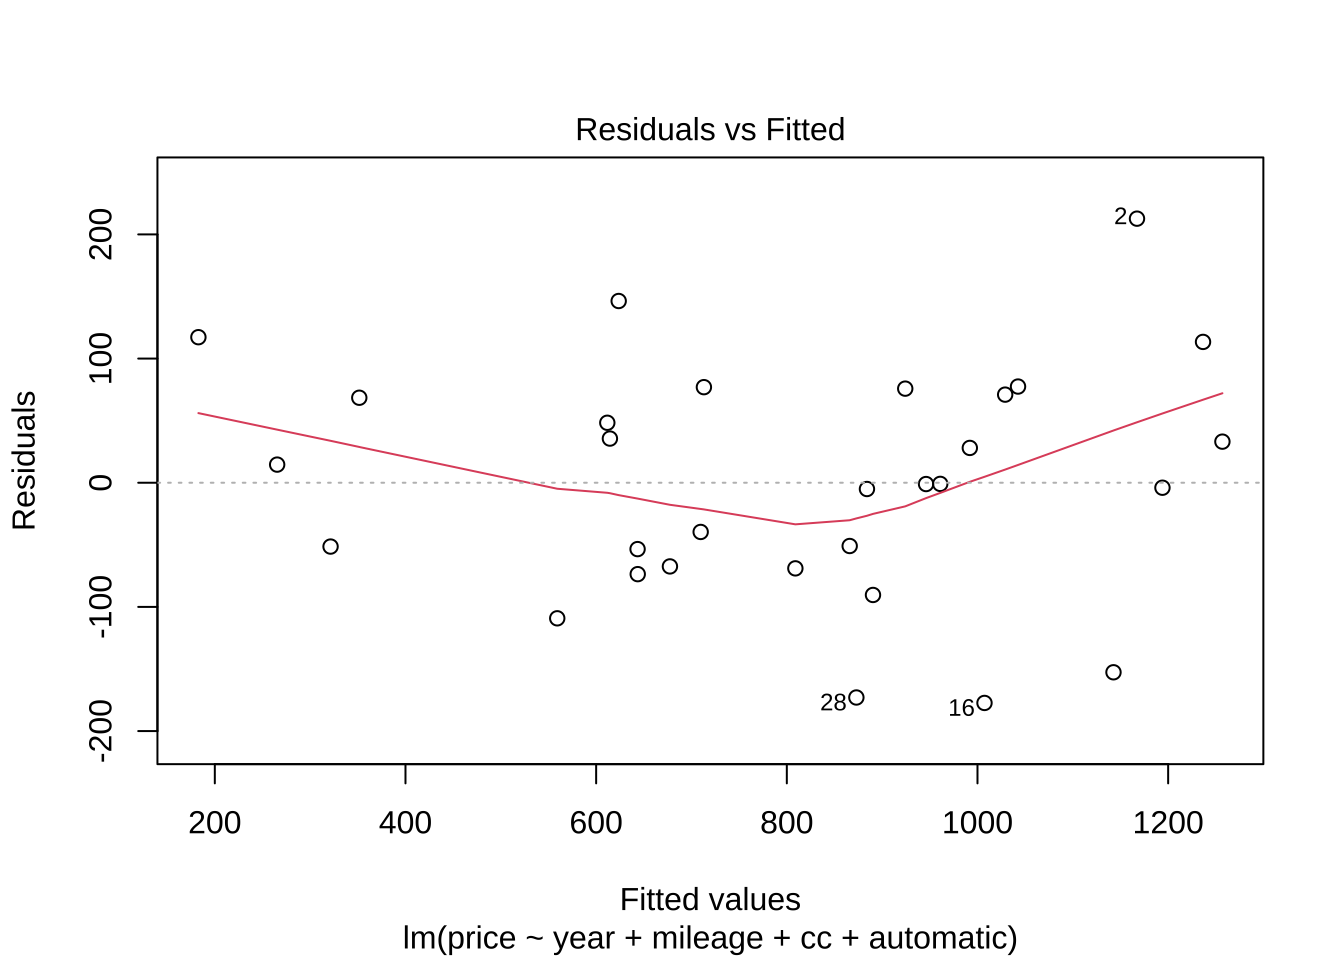
\includegraphics{qmd/lse_files/figure-pdf/unnamed-chunk-3-1.pdf}

위와 같은 자료를 이용하여 자동차의 속도가 주어졌을 경우 제동거리를
예측하려고 한다면 어떤 방법을 사용해야 할까?

\end{example}

\begin{example}[아파트
판매가격]\protect\hypertarget{exm-lse-simple-2}{}\label{exm-lse-simple-2}

다음 살펴볼 자료는 2019년 거래된 서울 아파트의 실거래 데이터 중 4개의
구(동대문구, 서초구, 관악구, 노원구)에서 거래된 아파트 중 1000개의
아파트를 임의로 추출한 자료이다.

\begin{Shaded}
\begin{Highlighting}[]
\NormalTok{apart\_2019 }\OtherTok{\textless{}{-}} \FunctionTok{read.csv}\NormalTok{(}\FunctionTok{here}\NormalTok{(}\StringTok{"data"}\NormalTok{, }\StringTok{"seoul\_apartment\_2019\_sample.csv"}\NormalTok{), }\AttributeTok{header =}\NormalTok{ T)}
\FunctionTok{head}\NormalTok{(apart\_2019,}\DecValTok{10}\NormalTok{)}
\end{Highlighting}
\end{Shaded}

\begin{verbatim}
       gu year  area price
1  관악구 1974 65.09   450
2  관악구 1978 56.86   276
3  관악구 1982 91.24   599
4  관악구 1982 91.24   560
5  관악구 1984 60.27   425
6  관악구 1984 60.27   420
7  관악구 1985 38.92   217
8  관악구 1988 61.74   485
9  관악구 1991 71.90   328
10 관악구 1991 84.44   438
\end{verbatim}

아파트의 면적(\texttt{area};제곱미터)에 따른
거래가격(\texttt{price};백만원)의 변화는 다음 그림과 같다.

\begin{Shaded}
\begin{Highlighting}[]
\FunctionTok{ggplot}\NormalTok{(apart\_2019, }\FunctionTok{aes}\NormalTok{(}\AttributeTok{x=}\NormalTok{area, }\AttributeTok{y=}\NormalTok{price)) }\SpecialCharTok{+} \FunctionTok{geom\_point}\NormalTok{() }\SpecialCharTok{+} \FunctionTok{labs}\NormalTok{(}\AttributeTok{x =} \StringTok{"면적(제곱미터)"}\NormalTok{, }\AttributeTok{y =} \StringTok{"거래가격(백만원)"}\NormalTok{) }\SpecialCharTok{+}
   \FunctionTok{labs}\NormalTok{(}\AttributeTok{title =} \StringTok{"아파트의 면적과 거래가격의 관계"}\NormalTok{)}
\end{Highlighting}
\end{Shaded}

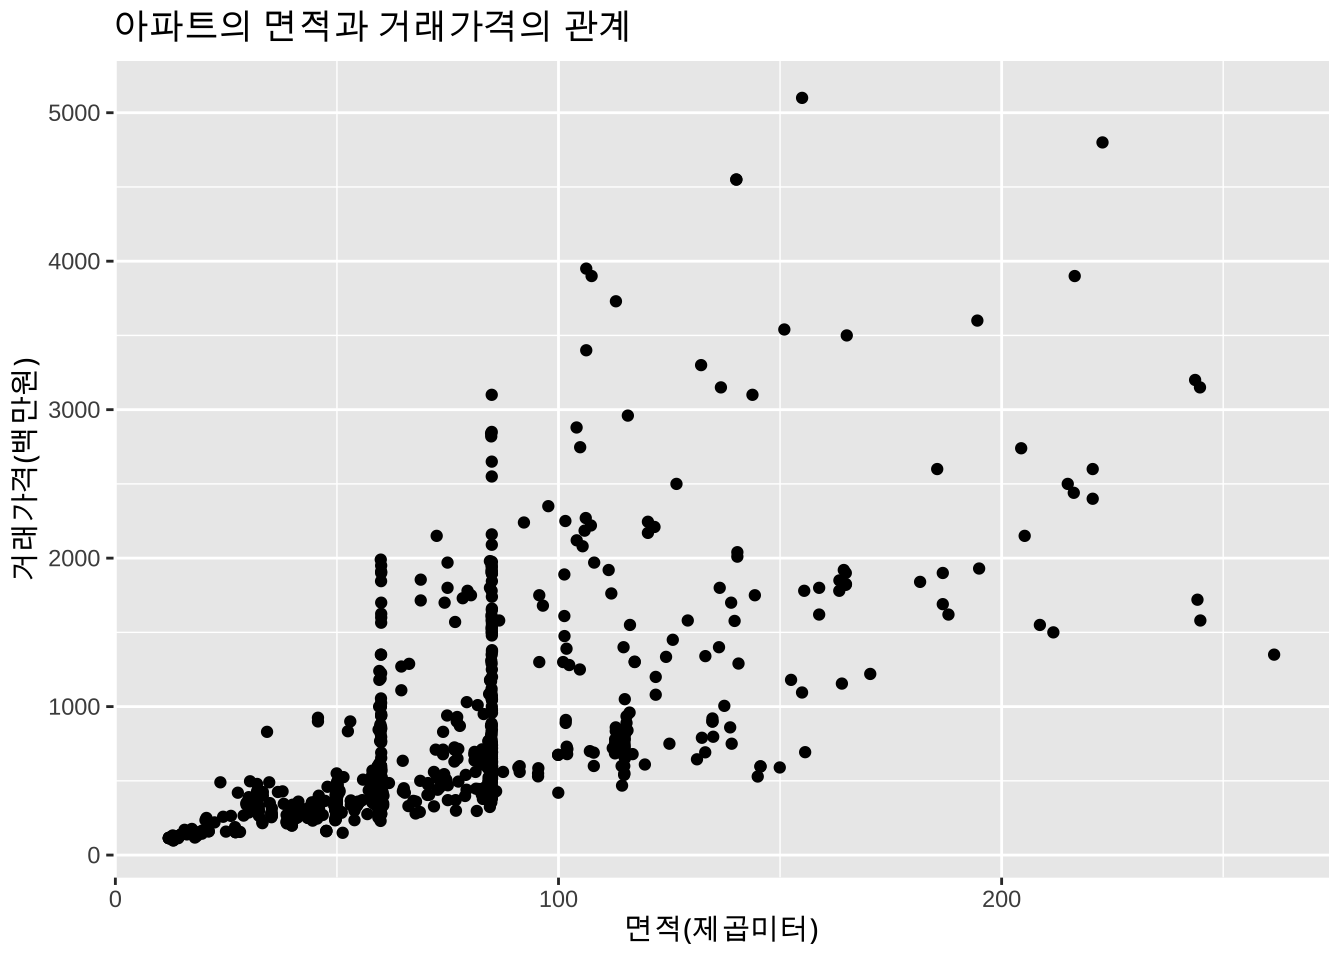
\includegraphics{qmd/lse_files/figure-pdf/unnamed-chunk-5-1.pdf}

만약 아파트의 면적(\texttt{x})과 거래가격(\texttt{y}) 대신 각각의
로그값(\texttt{log(x)}, `log(y))을 시용하면 다음과 같은 산포도가
나타난다.

\begin{Shaded}
\begin{Highlighting}[]
\CommentTok{\# log scale for y}
\FunctionTok{ggplot}\NormalTok{(apart\_2019, }\FunctionTok{aes}\NormalTok{(}\AttributeTok{x=}\NormalTok{area, }\AttributeTok{y=}\NormalTok{price)) }\SpecialCharTok{+} \FunctionTok{geom\_point}\NormalTok{() }\SpecialCharTok{+} \FunctionTok{labs}\NormalTok{(}\AttributeTok{x =} \StringTok{"면적(제곱미터)"}\NormalTok{, }\AttributeTok{y =} \StringTok{"거래가격(백만원)"}\NormalTok{) }\SpecialCharTok{+}
  \FunctionTok{scale\_y\_log10}\NormalTok{() }\SpecialCharTok{+} 
  \FunctionTok{scale\_x\_log10}\NormalTok{() }\SpecialCharTok{+}
  \FunctionTok{labs}\NormalTok{(}\AttributeTok{title =} \StringTok{"아파트의 면적과 거래가격의 관계 (로그스케일)"}\NormalTok{)}
\end{Highlighting}
\end{Shaded}

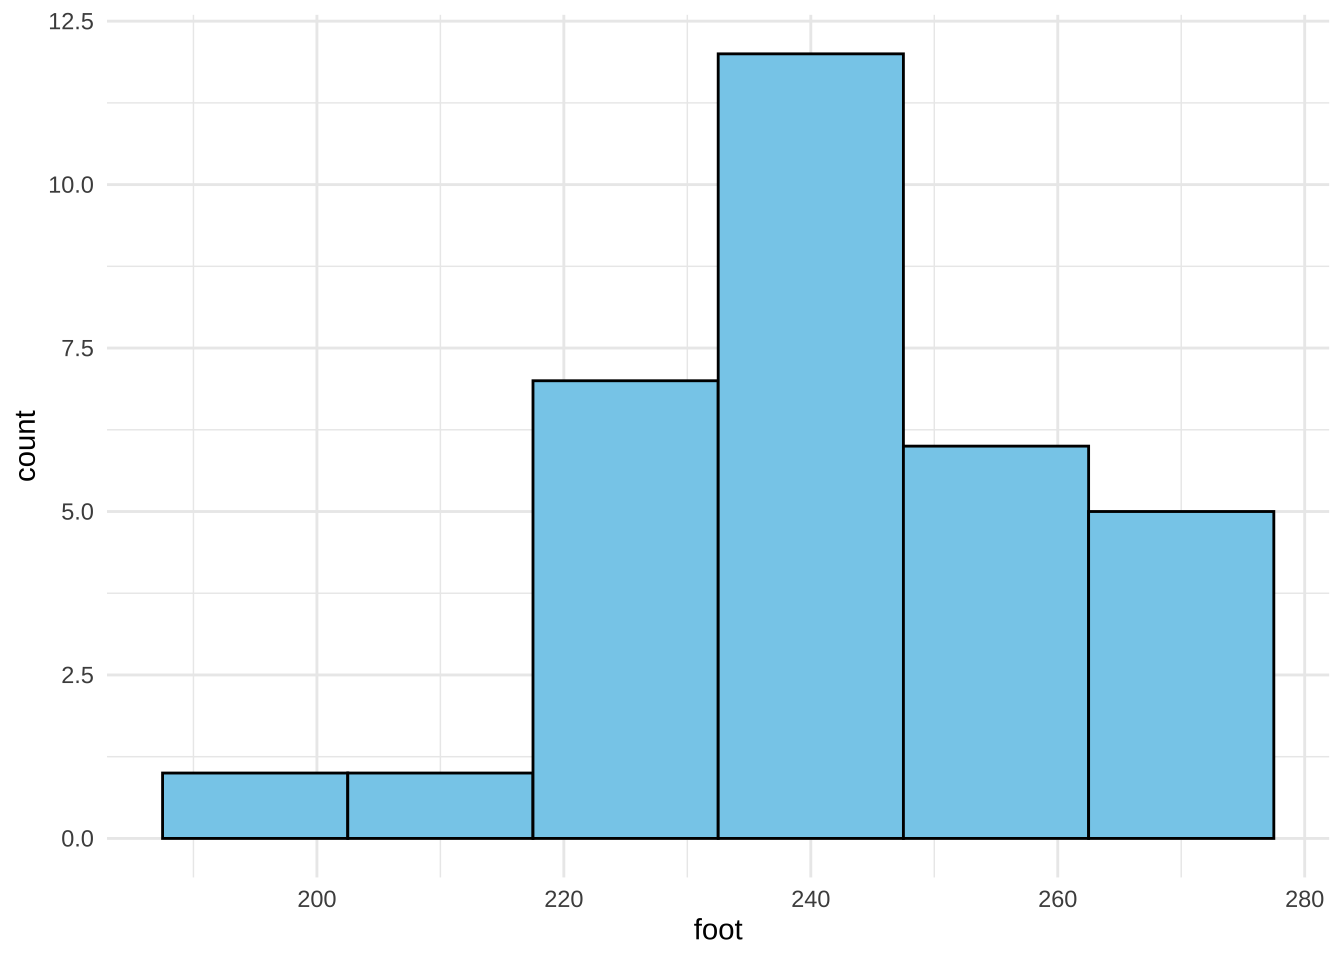
\includegraphics{qmd/lse_files/figure-pdf/unnamed-chunk-6-1.pdf}

\end{example}

\section{선형 회귀모형}\label{uxc120uxd615-uxd68cuxadc0uxbaa8uxd615}

회귀모형(regression model)는 변수들의 함수적 관계를 분석하는 통계적
방법이다. 일반적으로 한 개 또는 여러 개의 설명변수들(explanatory
variables, \texttt{x})이 관심있는 반응변수(response variable,
\texttt{y})에 어떤 형태로 영향을 미치는지에 파악하고 설명변수와
반응변수의 함수 관계를 통계적으로 추론하는 것이 회귀분석의 목적이다.

위에서 살펴본 두 예제에서 자동차의 속도(\texttt{x})가 증가하면
제동거리(\texttt{y})가 증가하는 경향이 있다는 것을 알 수 있으며,
아파트의 면적(\texttt{x})과 거래가격(\texttt{y})도 유사한 관계임을 알 수
있다.

이러한 두 변수의 관계를 다음과 같은 반응변수 \(y\) 와 설명변수의 선형
에측식(linear predictor)으로 나타내어 보자. 이러한 관계는 반응변수의
값의 변화를 근사적으로 설명변수의 선형식으로 예측할 수 있다는 의미이다.

\[ y \approx \beta_0 + \beta_1 x \]

위와 같은 근사적인 관계를 더 구체화하여 다음과 같이 반응변수의 평균값이
설명변수의 선형식으로 나타나는 것을 가정할 수 있으며 이를 선형
회귀모형(linear regression model)이라고 한다.이

\begin{equation}\phantomsection\label{eq-linreg01}{
E(y|x) = \beta_0 + \beta_1 x
}\end{equation}

식~\ref{eq-linreg01} 은 반응변수 \(y\)의 평균이 설명변수 \(x\) 의 선형
예측식으로 나타나는 관계를 가정한 것이며 절편 \(\beta_0\) 와 기울기
\(\beta_1\) 는 회귀계수(regression coefficient)라고 부르는
모수(parameter)로서 추정해야 한다.

특별히 하나의 설명변수를 사용하는 회귀 모형을 단순선형 회귀모형(simple
linear regression model)이라고 한다.

위에서 본 두 예제와 같이 \(n\) 개의 자료
\((x_1,y_1),(x_2,y_2),..,(x_n, y_n)\)을 독립적으로 추출하였다면 자료의
생성 과정을 다음과 같은 단순선형 회귀모형으로 나타낼 수 있다. 반응변수
\(y_i\)는 설명변수 \(x_i\)의 선형함수로 표현된 선형 예측식
식~\ref{eq-linreg01} 과 임의의 오차항 (random error) \(e_i\) 의 합으로
나타내어진다고 가정하자.

\begin{equation}\phantomsection\label{eq-linreg02}{
y_i = \beta_0 + \beta_1 x_i + e_i, \quad i=1,2,\dots,n
}\end{equation}

여기서 오차항 \(e_i\)는 평균이 \(0\)이고 분산이 \(\sigma^2\) 인 임의의
확률분포를 따르며 서로 독립이라고 가정한다.

\[ E(e_i)=0, \quad V(e_i) = \sigma^2 \quad i=1,2,\dots,n \]

오차항의 분산 \(\sigma^2\)도 추정해야할 모수(parameter)이다.

\section{최소제곱법}\label{uxcd5cuxc18cuxc81cuxacf1uxbc95}

앞에서 언급한 것과 같이 선형회귀모형 식~\ref{eq-linreg02} 에서 모수
\(\beta_0\)와 \(\beta_1\)를 회귀계수라고 하며 자료를 이용하여 추정해야
한다. \(n\)개의 자료를 이용하여 회귀계수 \(\beta_0\)와 \(\beta_1\)를
추정하려고 할 때 사용할 수 있는 방법들 중에서 가장 쉽고 유용한 방법은
최소제곱법(least square method)이다.

회귀모형 식~\ref{eq-linreg02} 에서 \(\beta_0\)와 \(\beta_1\)의 값이
주어졌다면 설명변수 \(x_i\) 에서 반응변수의 관측값 \(y_i\)에 가장
합리적인 예측값은 무었일까? 가장 합리적인 예측값은 주어진 \(x_i\)에서
반응변수의 평균값인 \(E(y_i | x_i)=\beta_0 + \beta_1 x_i\)이다. 여기서
실제 관측하여 얻어진 값 \(y_i\)와 예측값 \(\beta_0 + \beta_1 x_i\)
사이에는 오차에 의해서 차이가 발생할 수 있다. 그 차이를
잔차(residual)라고 하며 \(r_i\) 라고 표기한다.

\[  r_i = y_i - E(y_i|x_i) = y_i - (  \beta_0 +  \beta_1 x_i) \]

잔차는 위에 식에서 알 수 있듯이 관측값과 회귀식을 통한 예측값의 차이를
나타낸 것이다. 그러면 자료를 가장 잘 설명할 수 있는 회귀직선을 얻기
위해서는 잔차 \(r_i\)를 가장 작게하는 회귀모형을 세워야 한다. 잔차들을
최소로 하는 방법들 중 하나인 최소제곱법은 잔차들의 제곱합을 최소로 하는
회귀계수 \(\beta_0\)와 \(\beta_1\)를 추정하는 방법이다. 잔차들의
제곱합은 다음과 같이 표현된다.

\begin{equation}\phantomsection\label{eq-rsq}{
 S(\beta_0 , \beta_1) = \sum^n_{i=1}r^2_i = \sum^n_{i=1}[y_i-(\beta_0 + \beta_1 x_i)]^2 
}\end{equation}

\begin{tcolorbox}[enhanced jigsaw, colback=white, title=\textcolor{quarto-callout-note-color}{\faInfo}\hspace{0.5em}{노트}, colbacktitle=quarto-callout-note-color!10!white, toprule=.15mm, breakable, bottomtitle=1mm, left=2mm, colframe=quarto-callout-note-color-frame, leftrule=.75mm, coltitle=black, toptitle=1mm, titlerule=0mm, arc=.35mm, opacityback=0, opacitybacktitle=0.6, rightrule=.15mm, bottomrule=.15mm]

식~\ref{eq-rsq} 를 잔차제곱합(residusl sum of square)이라고 부른다.
일반적으로 회귀계수의 값이 특정지어져서 실제로 잔차를 계산할 수 있는
경우 잔차제곱합이라고 부른다. 뒤에 분산분석에서는 잔차제곱합을 SSE(sum
of square error)라고 부른다.

잔차제곱합을 최소로 하는 회귀계수의 값을 찾는 최적화의 목표로
잔차제곱합이 제시될 때 이를 오차제곱합(error sum of square)이라고
부른다.

\end{tcolorbox}

위의 오차제곱합 \(S(\beta_0 , \beta_1)\) 을 최소화하는 \(\beta_0\)와
\(\beta_1\)의 값을 구하는 방법은 오차제곱합이 \(\beta_0\)와
\(\beta_1\)의 미분 가능한 2차 함수이고 아래로 볼록한 함수(convex
function)임을 이용한다.

\begin{Shaded}
\begin{Highlighting}[]
\NormalTok{gridnum }\OtherTok{\textless{}{-}} \DecValTok{60}
\NormalTok{sizing }\OtherTok{\textless{}{-}} \DecValTok{5}
\NormalTok{extrascale }\OtherTok{\textless{}{-}} \DecValTok{10}
\NormalTok{extrascale2 }\OtherTok{\textless{}{-}} \FloatTok{0.7}
\NormalTok{b0 }\OtherTok{\textless{}{-}} \FunctionTok{seq}\NormalTok{(}\SpecialCharTok{{-}}\FloatTok{17.6}\SpecialCharTok{{-}}\NormalTok{sizing}\SpecialCharTok{*}\NormalTok{extrascale,  }\SpecialCharTok{{-}}\FloatTok{17.6}\SpecialCharTok{+}\NormalTok{sizing}\SpecialCharTok{*}\NormalTok{extrascale, }\AttributeTok{length=}\NormalTok{gridnum )}
\NormalTok{b1 }\OtherTok{\textless{}{-}} \FunctionTok{seq}\NormalTok{(}\DecValTok{4}\SpecialCharTok{{-}}\NormalTok{sizing}\SpecialCharTok{*}\NormalTok{extrascale2, }\DecValTok{4}\SpecialCharTok{+}\NormalTok{sizing}\SpecialCharTok{*}\NormalTok{extrascale2, }\AttributeTok{length=}\NormalTok{gridnum )}

\NormalTok{SSE }\OtherTok{\textless{}{-}} \FunctionTok{matrix}\NormalTok{(}\DecValTok{0}\NormalTok{, gridnum, gridnum )}
\ControlFlowTok{for}\NormalTok{ (i }\ControlFlowTok{in} \DecValTok{1}\SpecialCharTok{:}\NormalTok{gridnum ) \{}
  \ControlFlowTok{for}\NormalTok{ (j }\ControlFlowTok{in} \DecValTok{1}\SpecialCharTok{:}\NormalTok{gridnum )\{}
\NormalTok{    r }\OtherTok{\textless{}{-}}\NormalTok{ cars}\SpecialCharTok{$}\NormalTok{dist}\SpecialCharTok{{-}}\NormalTok{ b0[i] }\SpecialCharTok{{-}}\NormalTok{b1[j]}\SpecialCharTok{*}\NormalTok{cars}\SpecialCharTok{$}\NormalTok{speed}
\NormalTok{    SSE[i,j]  }\OtherTok{\textless{}{-}}\NormalTok{ (}\FunctionTok{sum}\NormalTok{(r}\SpecialCharTok{\^{}}\DecValTok{2}\NormalTok{))}\SpecialCharTok{/}\DecValTok{1000}
\NormalTok{  \}}
\NormalTok{\}}

\FunctionTok{persp3D}\NormalTok{(b0, b1, SSE, }\AttributeTok{theta =}\DecValTok{10}\NormalTok{, }\AttributeTok{phi =} \DecValTok{20}\NormalTok{, }\AttributeTok{expand =} \DecValTok{1}\NormalTok{)}
\end{Highlighting}
\end{Shaded}

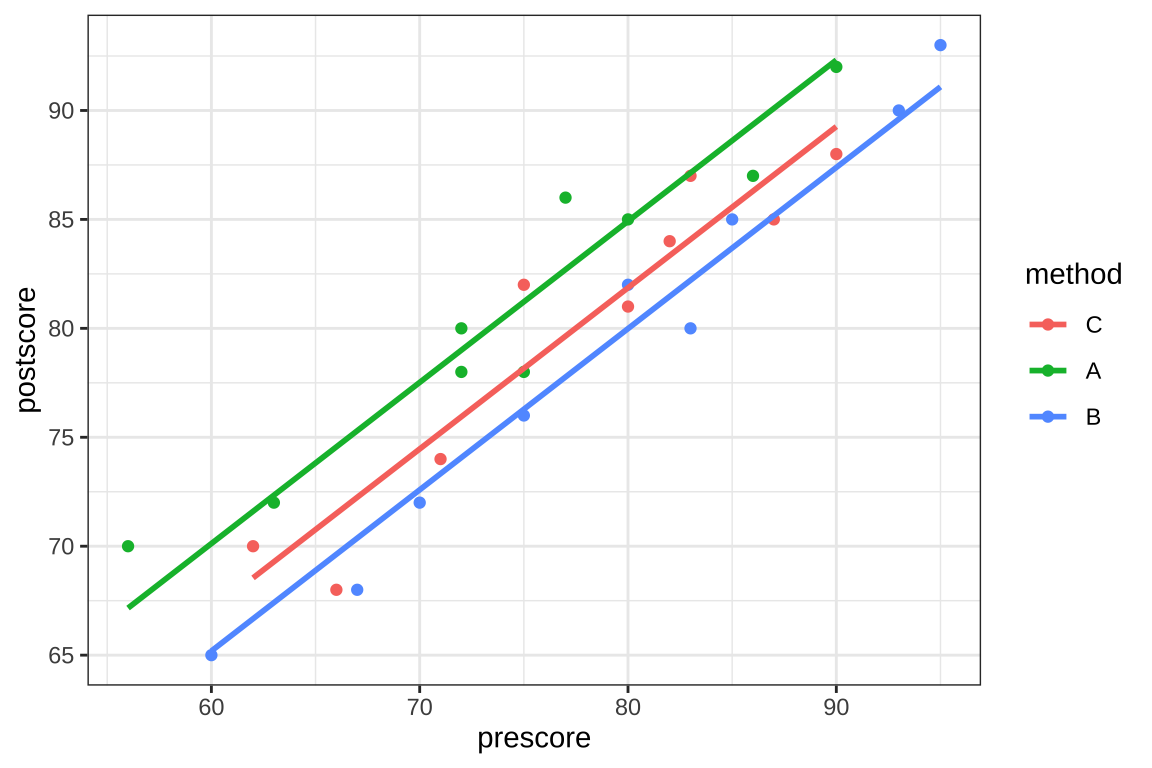
\includegraphics{qmd/lse_files/figure-pdf/unnamed-chunk-7-1.pdf}

\begin{Shaded}
\begin{Highlighting}[]
\DocumentationTok{\#\# Interactive 3d graph}
\CommentTok{\#fig \textless{}{-} plot\_ly(z = \textasciitilde{}SSE)}
\CommentTok{\#fig \textless{}{-} fig \%\textgreater{}\% add\_surface()}
\CommentTok{\#fig}
\end{Highlighting}
\end{Shaded}

위의 그림을 보면 볼록한 모양이 너무 평평하여 오차제곱합이 최소가 되는
\(\beta_0\)와 \(\beta_1\)의 위치가 명확하지 않다.

이제 모든 변수들을 표준화하고 표준화된 변수들에 단순회귀모형에 대한
오차제곱합을 \(\beta_0\)와 \(\beta_1\)의 함수로서 그림을 그리면 아래와
같다.

\begin{equation}\phantomsection\label{eq-linreg02-std}{ 
v_i = \beta_0 + \beta_1 w_i + e_i, \quad i=1,2,\dots,n 
}\end{equation}

여기서

\[ v_i  = \frac{y_i -\bar y}{s_y}, \quad w_i = \frac{x_i -\bar x}{s_x} \]

\begin{Shaded}
\begin{Highlighting}[]
\CommentTok{\# 변수들을 표준화!}
\NormalTok{std\_cars }\OtherTok{\textless{}{-}} \FunctionTok{as.data.frame}\NormalTok{(}\FunctionTok{scale}\NormalTok{(cars))}
\NormalTok{gridnum }\OtherTok{\textless{}{-}} \DecValTok{60}
\NormalTok{sizing }\OtherTok{\textless{}{-}} \DecValTok{1}
\NormalTok{b0 }\OtherTok{\textless{}{-}} \FunctionTok{seq}\NormalTok{(}\DecValTok{0}\SpecialCharTok{{-}}\NormalTok{sizing,  }\DecValTok{0}\SpecialCharTok{+}\NormalTok{sizing, }\AttributeTok{length=}\NormalTok{gridnum )}
\NormalTok{b1 }\OtherTok{\textless{}{-}} \FunctionTok{seq}\NormalTok{(}\DecValTok{1}\SpecialCharTok{{-}}\NormalTok{sizing, }\DecValTok{1}\SpecialCharTok{+}\NormalTok{sizing, }\AttributeTok{length=}\NormalTok{gridnum )}

\NormalTok{SSE }\OtherTok{\textless{}{-}} \FunctionTok{matrix}\NormalTok{(}\DecValTok{0}\NormalTok{, gridnum, gridnum )}
\ControlFlowTok{for}\NormalTok{ (i }\ControlFlowTok{in} \DecValTok{1}\SpecialCharTok{:}\NormalTok{gridnum ) \{}
  \ControlFlowTok{for}\NormalTok{ (j }\ControlFlowTok{in} \DecValTok{1}\SpecialCharTok{:}\NormalTok{gridnum )\{}
\NormalTok{    r }\OtherTok{\textless{}{-}}\NormalTok{ std\_cars}\SpecialCharTok{$}\NormalTok{dist}\SpecialCharTok{{-}}\NormalTok{ b0[i] }\SpecialCharTok{{-}}\NormalTok{b1[j]}\SpecialCharTok{*}\NormalTok{std\_cars}\SpecialCharTok{$}\NormalTok{speed}
\NormalTok{    SSE[i,j]  }\OtherTok{\textless{}{-}} \FunctionTok{sum}\NormalTok{(r}\SpecialCharTok{\^{}}\DecValTok{2}\NormalTok{)}
\NormalTok{  \}}
\NormalTok{\}}

\FunctionTok{persp3D}\NormalTok{(b0, b1, SSE, }\AttributeTok{theta =}\DecValTok{40}\NormalTok{, }\AttributeTok{phi =} \DecValTok{15}\NormalTok{, }\AttributeTok{expand =} \DecValTok{1}\NormalTok{)}
\end{Highlighting}
\end{Shaded}

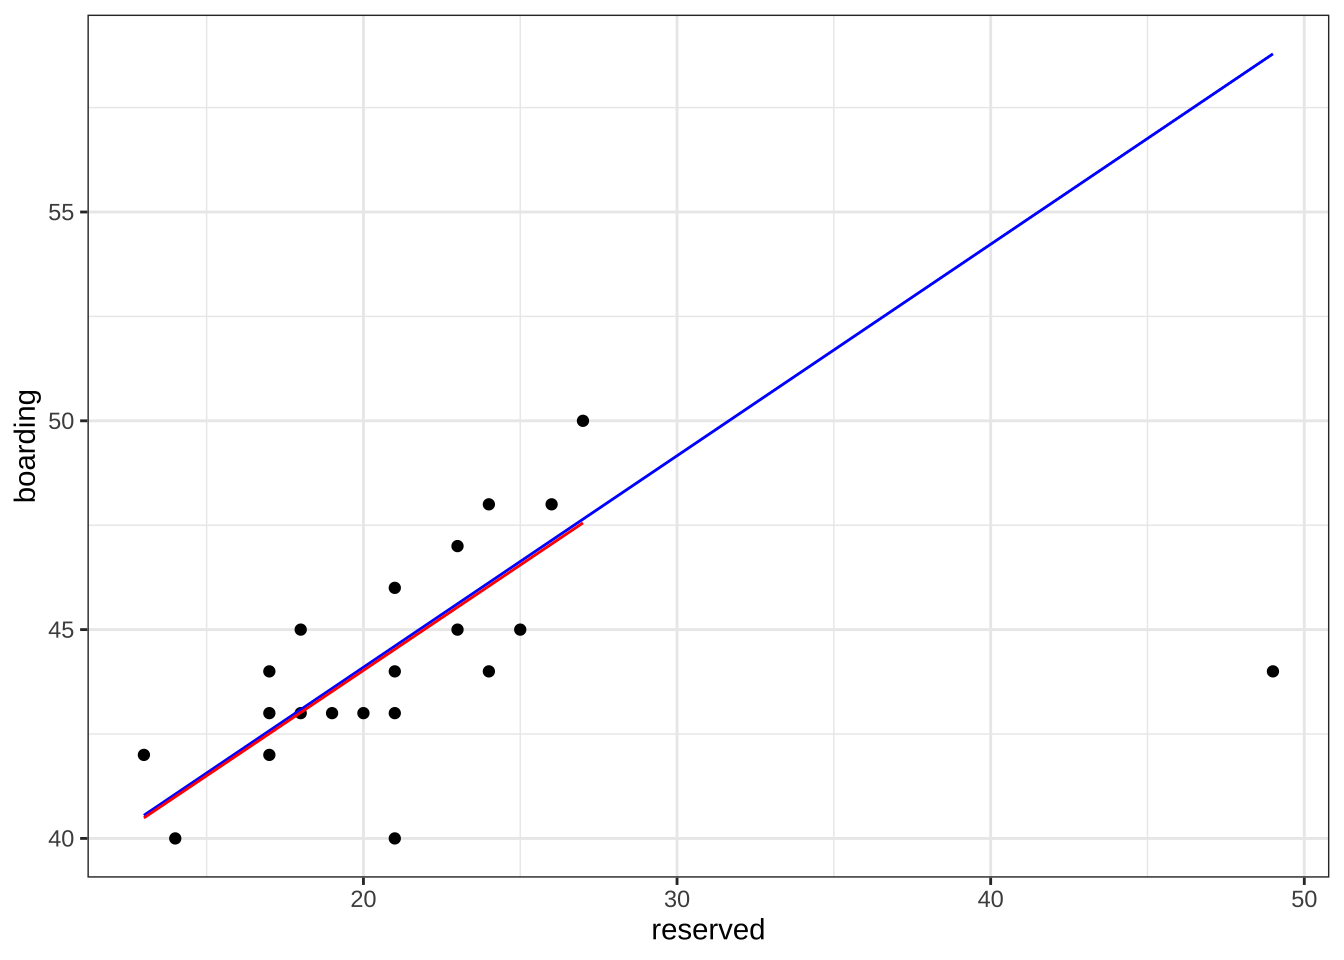
\includegraphics{qmd/lse_files/figure-pdf/unnamed-chunk-8-1.pdf}

\begin{Shaded}
\begin{Highlighting}[]
\DocumentationTok{\#\# Interactive 3d graph}
\CommentTok{\#fig \textless{}{-} plot\_ly(z = \textasciitilde{}SSE)}
\CommentTok{\#fig \textless{}{-} fig \%\textgreater{}\% add\_surface()}
\CommentTok{\#fig}
\end{Highlighting}
\end{Shaded}

위위 같이 변수들을 표준화하면 오차제곱합 함수의 볼록한 정도가 덜
평평하게 변하여 최적값을 더 확실하게 보인다. 기계학습이나 인공지능
모형에서 적합하기 전에 모든 변수를 표준화하는 이유가 위의 그림에서
나타난다.

식~\ref{eq-rsq} 의 오차제곱합을 각 회귀계수에 대해서 편미분을 하고 0으로
놓으면 아래와 같이 두 방정식이 얻어진다.

\begin{equation}\phantomsection\label{eq-normaleq02}{
\begin{aligned}
 \pardiff{ S(\beta_0 , \beta_1)}{\beta_0} & = \sum^n_{i=1}(-2)[y_i-(\beta_0+\beta_1 x_i)]=0    \\ \notag 
\pardiff{ S(\beta_0 , \beta_1)}{\beta_1}  & = \sum^n_{i=1}(-2 x_i)[y_i-(\beta_0+\beta_1 x_i)]=0 
\end{aligned}
}\end{equation}

위의 연립방정식을 행렬식으로 표시하면 다음과 같이 나타낼 수 있다.

\[ 
\begin{bmatrix}
n & \sum_i x_i \\
\sum_i x_i & \sum_i x^2_i
\end{bmatrix}
\begin{bmatrix}
\beta_0 \\
\beta_1
\end{bmatrix}
=
\begin{bmatrix}
\sum_i y_i \\
\sum_i x_i y_i
\end{bmatrix}
\]

위의 방정식을 풀어서 구한 회귀계수의 추정치를 \(\hat \beta_0\),
\(\hat \beta_1\) 이라고 하면 다음과 같이 주어진다.

\begin{align*}
 \hat \beta_0 &= \bar y - \hat \beta_1 \bar x  \\ 
  \hat \beta_1 &=  \frac{ \sum_i (x_i - \bar x)(y_i - \bar y)}{\sum_i (x_i - \bar x)^2} 
\end{align*}

최소제곱법에서 얻어진 회귀계수의 추정량 \(\hat \beta_0\)과
\(\hat \beta_1\) 을 이용한 반응변수 \(y_i\) 에 대한 예측값
\(\hat y_i\)는 다음과 같이 정의되고

\[ \hat y_i = \hat E(y_i|x_i) = \hat \beta_0 + \hat \beta_1 x_i \]

\begin{tcolorbox}[enhanced jigsaw, colback=white, title=\textcolor{quarto-callout-caution-color}{\faFire}\hspace{0.5em}{표준화 전과 후}, colbacktitle=quarto-callout-caution-color!10!white, toprule=.15mm, breakable, bottomtitle=1mm, left=2mm, colframe=quarto-callout-caution-color-frame, leftrule=.75mm, coltitle=black, toptitle=1mm, titlerule=0mm, arc=.35mm, opacityback=0, opacitybacktitle=0.6, rightrule=.15mm, bottomrule=.15mm]

두 개의 회귀방정식 식~\ref{eq-linreg02} 과 식~\ref{eq-linreg02-std} 에서
각각 최소제곱법으로 구한 기울기의 추정치 \(\hat \beta_1\) 이 동일하게
나타나는 경우는 어떤 경우일까 생각해보자.

\end{tcolorbox}

잔차 \(r_i\)는 다음과 같이 계산한다.

\begin{equation}\phantomsection\label{eq-residual}{
r_i = y_i - (\hat \beta_0 + \hat \beta_1 x_i) = y_i -\hat y_i  
}\end{equation}

잔차 \(r_i\)는 다음과 같은 성질을 가진다.

\[ \sum_{i=1}^n r_i = 0 \]

\[ \sum_{i=1}^n x_i r_i = 0 \]

이제 위에서 본 \texttt{cars} 자료를 가지고 선형회귀모형
식~\ref{eq-linreg02} 에 나타난 회귀계수를 추정해보자. 아래는 \texttt{R}
프로그램에서 함수 \texttt{lm}을 이용한 추정결과이다.

\begin{Shaded}
\begin{Highlighting}[]
\NormalTok{lm\_car }\OtherTok{\textless{}{-}} \FunctionTok{lm}\NormalTok{(dist}\SpecialCharTok{\textasciitilde{}}\NormalTok{speed, }\AttributeTok{data=}\NormalTok{cars)}
\FunctionTok{summary}\NormalTok{(lm\_car)}
\end{Highlighting}
\end{Shaded}

\begin{verbatim}

Call:
lm(formula = dist ~ speed, data = cars)

Residuals:
    Min      1Q  Median      3Q     Max 
-29.069  -9.525  -2.272   9.215  43.201 

Coefficients:
            Estimate Std. Error t value Pr(>|t|)    
(Intercept) -17.5791     6.7584  -2.601   0.0123 *  
speed         3.9324     0.4155   9.464 1.49e-12 ***
---
Signif. codes:  0 '***' 0.001 '**' 0.01 '*' 0.05 '.' 0.1 ' ' 1

Residual standard error: 15.38 on 48 degrees of freedom
Multiple R-squared:  0.6511,    Adjusted R-squared:  0.6438 
F-statistic: 89.57 on 1 and 48 DF,  p-value: 1.49e-12
\end{verbatim}

위에서 주어진 선형회귀모형 식~\ref{eq-linreg02} 에 대한 추정 결과를
이용하면 자동차의 속도(\(x\) = \texttt{speed})와 제동거리(\(y\) =
\texttt{dist})의 관계는 다음과 같은 회귀식으로 나타낼 수 있다.

\[ \hat E(y | x) = −17.58 + 3.93 x \]

\begin{Shaded}
\begin{Highlighting}[]
\FunctionTok{ggplot}\NormalTok{(cars, }\FunctionTok{aes}\NormalTok{(}\AttributeTok{x=}\NormalTok{speed, }\AttributeTok{y=}\NormalTok{dist)) }\SpecialCharTok{+} \FunctionTok{geom\_point}\NormalTok{() }\SpecialCharTok{+} \FunctionTok{labs}\NormalTok{(}\AttributeTok{x =} \StringTok{"속도"}\NormalTok{, }\AttributeTok{y =} \StringTok{"거리"}\NormalTok{) }\SpecialCharTok{+}
  \FunctionTok{labs}\NormalTok{(}\AttributeTok{title=}\StringTok{"자동차의 속도와 제동거리의 관계"}\NormalTok{) }\SpecialCharTok{+} 
  \FunctionTok{geom\_abline}\NormalTok{(}\AttributeTok{intercept =} \SpecialCharTok{{-}}\FloatTok{17.58}\NormalTok{, }\AttributeTok{slope =} \FloatTok{3.93}\NormalTok{, }\AttributeTok{color =} \StringTok{"red"}\NormalTok{)}
\end{Highlighting}
\end{Shaded}

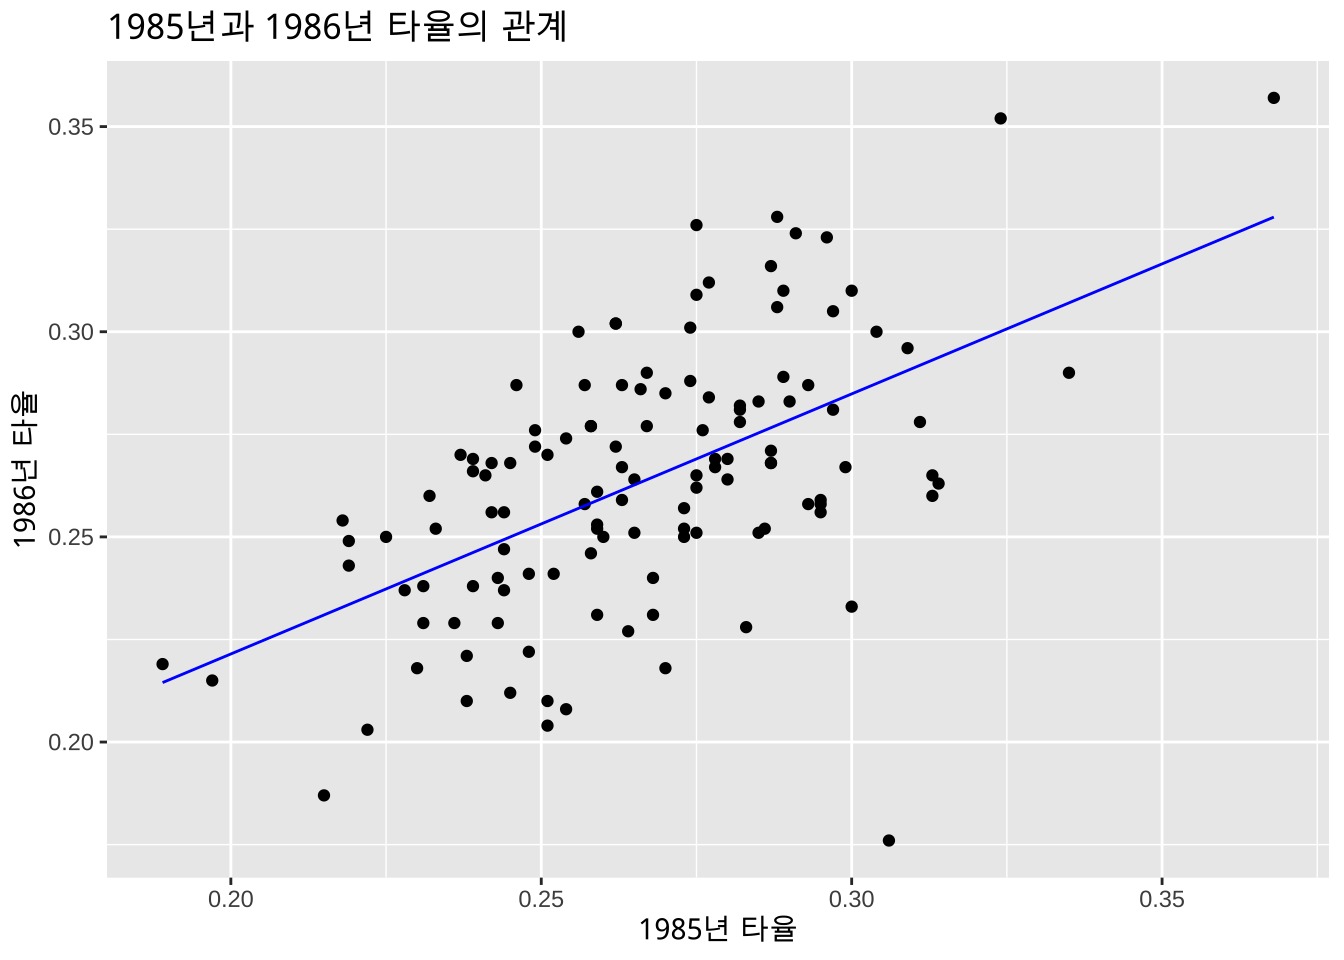
\includegraphics{qmd/lse_files/figure-pdf/unnamed-chunk-10-1.pdf}

위의 추정식을 이용하면 주어진 자동차의 속도에서 제동거리를 예측할 수
있다. 예를 들어 자동차의 속도가 25 mph인 경우에는 제동거리의 평균이
80.73 mph 임을 알 수 있다.

\[ E(y|x=25) = −17.58 + 3.93 (25) = 80.73 \]

\begin{Shaded}
\begin{Highlighting}[]
\NormalTok{newcars }\OtherTok{\textless{}{-}} \FunctionTok{data.frame}\NormalTok{(}\AttributeTok{speed =} \FunctionTok{c}\NormalTok{(}\DecValTok{25}\NormalTok{))}
\FunctionTok{predict}\NormalTok{(lm\_car, }\AttributeTok{newdata=}\NormalTok{newcars)}
\end{Highlighting}
\end{Shaded}

\begin{verbatim}
       1 
80.73112 
\end{verbatim}

기울기의 추정값 \(\hat \beta_1 = 3.93\) 은 자동차의 속도 (\(x\))가 1 mph
증가할 때 평균 제동거리 (\(E(y|x)\))가 3.93 ft 증가한다는 의미이다.

이제 아파트 거애 가격에 대한 단순선형회귀모형을 적합해보자. 이 경우
면적과 가격대신 각각의 로그값을 사용하여 회귀모형을 적합해 보자. 아래는
아파트의 면적과 거래가격에 대한 단순선형 회귀모형을 적합한 결과이다.

\begin{Shaded}
\begin{Highlighting}[]
\NormalTok{apart\_2019\_log }\OtherTok{\textless{}{-}}\NormalTok{ apart\_2019 }\SpecialCharTok{\%\textgreater{}\%} 
  \FunctionTok{mutate}\NormalTok{(}\AttributeTok{log\_area =} \FunctionTok{log10}\NormalTok{(area), }\AttributeTok{log\_price =} \FunctionTok{log10}\NormalTok{(price)) }\SpecialCharTok{\%\textgreater{}\%}
\NormalTok{  dplyr}\SpecialCharTok{::}\FunctionTok{select}\NormalTok{(log\_area, log\_price)}

\FunctionTok{head}\NormalTok{(apart\_2019\_log,}\DecValTok{10}\NormalTok{)}
\end{Highlighting}
\end{Shaded}

\begin{verbatim}
   log_area log_price
1  1.813514  2.653213
2  1.754807  2.440909
3  1.960185  2.777427
4  1.960185  2.748188
5  1.780101  2.628389
6  1.780101  2.623249
7  1.590173  2.336460
8  1.790567  2.685742
9  1.856729  2.515874
10 1.926548  2.641474
\end{verbatim}

\begin{Shaded}
\begin{Highlighting}[]
\NormalTok{lm\_apart }\OtherTok{\textless{}{-}} \FunctionTok{lm}\NormalTok{( log\_price}\SpecialCharTok{\textasciitilde{}}\NormalTok{ log\_area, }\AttributeTok{data=}\NormalTok{apart\_2019\_log)}
\FunctionTok{summary}\NormalTok{(lm\_apart)}
\end{Highlighting}
\end{Shaded}

\begin{verbatim}

Call:
lm(formula = log_price ~ log_area, data = apart_2019_log)

Residuals:
     Min       1Q   Median       3Q      Max 
-0.45348 -0.12132 -0.04075  0.07531  0.62358 

Coefficients:
            Estimate Std. Error t value Pr(>|t|)    
(Intercept)  0.76902    0.05217   14.74   <2e-16 ***
log_area     1.08797    0.02843   38.27   <2e-16 ***
---
Signif. codes:  0 '***' 0.001 '**' 0.01 '*' 0.05 '.' 0.1 ' ' 1

Residual standard error: 0.1894 on 998 degrees of freedom
Multiple R-squared:  0.5948,    Adjusted R-squared:  0.5944 
F-statistic:  1465 on 1 and 998 DF,  p-value: < 2.2e-16
\end{verbatim}

위의 결과는 다음과 같이 나타낼 수 있다.

\[ \hat E( \log10 y | x) = 0.769 + 1.0797 \log10 (x) \]

\begin{Shaded}
\begin{Highlighting}[]
\FunctionTok{ggplot}\NormalTok{(apart\_2019\_log, }\FunctionTok{aes}\NormalTok{(}\AttributeTok{x=}\NormalTok{log\_area, }\AttributeTok{y=}\NormalTok{log\_price)) }\SpecialCharTok{+} \FunctionTok{geom\_point}\NormalTok{() }\SpecialCharTok{+} \FunctionTok{labs}\NormalTok{(}\AttributeTok{x =} \StringTok{"로그 면적(제곱미터)"}\NormalTok{, }\AttributeTok{y =} \StringTok{"로그 거래가격(백만원)"}\NormalTok{) }\SpecialCharTok{+}
  \FunctionTok{labs}\NormalTok{(}\AttributeTok{title =} \StringTok{"아파트의 면적과 거래가격의 관계 (로그스케일)"}\NormalTok{) }\SpecialCharTok{+} 
  \FunctionTok{geom\_abline}\NormalTok{(}\AttributeTok{intercept =} \FloatTok{0.769}\NormalTok{, }\AttributeTok{slope =} \FloatTok{1.0797}\NormalTok{, }\AttributeTok{color =} \StringTok{"red"}\NormalTok{)}
\end{Highlighting}
\end{Shaded}

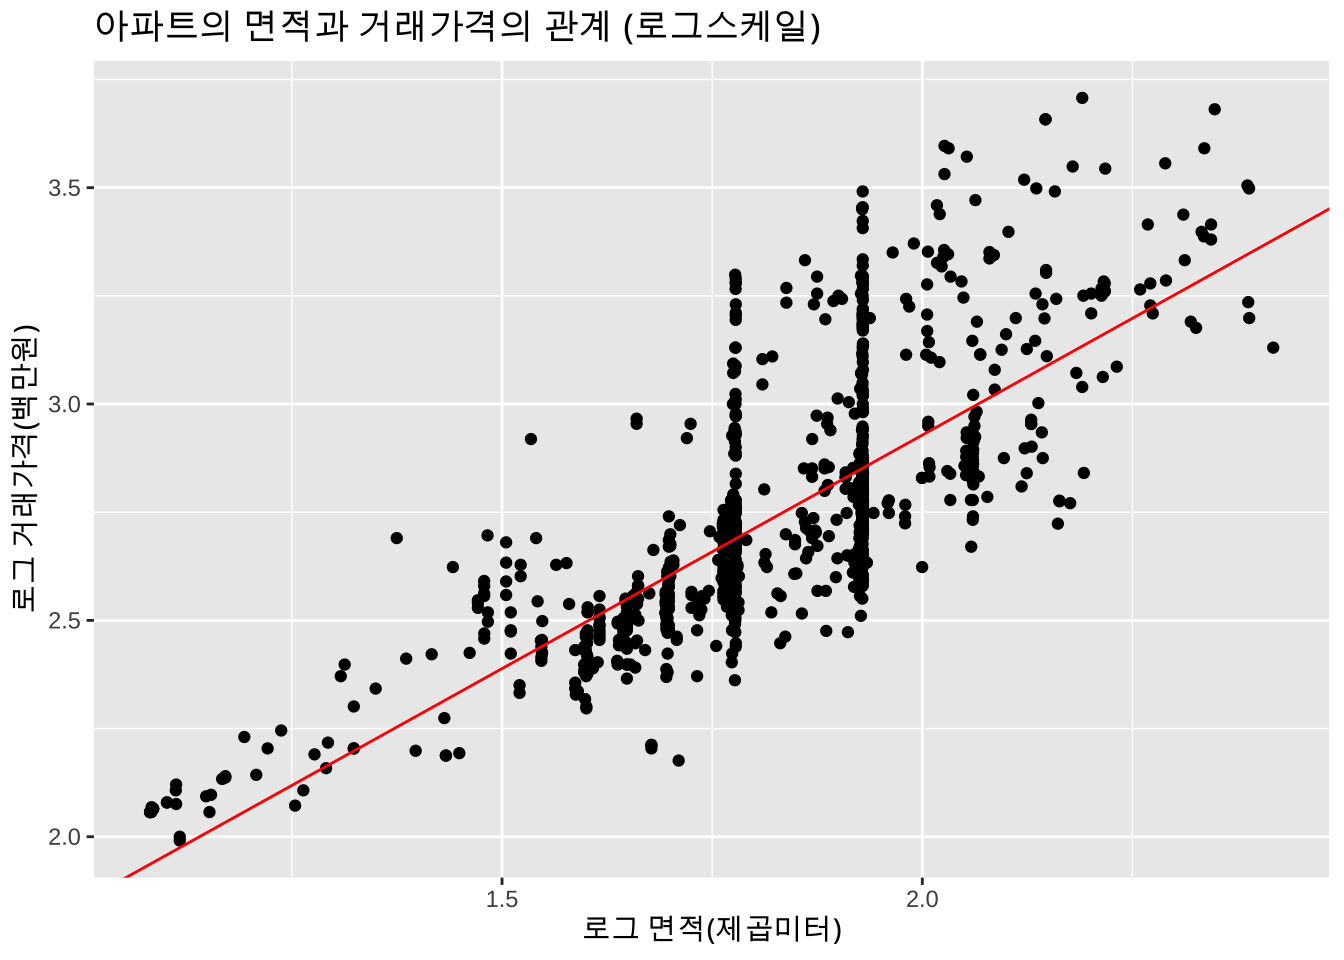
\includegraphics{qmd/lse_files/figure-pdf/unnamed-chunk-14-1.pdf}

이제 위의 결과를 응용하면 아파트의 면적이 100 제곱미터인 경우의 아파트의
평균 거래가격을 880(백만원)으로 예측할 수 있다.

\begin{Shaded}
\begin{Highlighting}[]
\NormalTok{newapart }\OtherTok{\textless{}{-}} \FunctionTok{data.frame}\NormalTok{(}\AttributeTok{log\_area =} \FunctionTok{c}\NormalTok{(}\FunctionTok{log10}\NormalTok{(}\DecValTok{100}\NormalTok{)))}
\NormalTok{pred\_y }\OtherTok{\textless{}{-}} \DecValTok{10}\SpecialCharTok{\^{}}\FunctionTok{predict}\NormalTok{(lm\_apart, }\AttributeTok{newdata=}\NormalTok{newapart)}
\NormalTok{pred\_y}
\end{Highlighting}
\end{Shaded}

\begin{verbatim}
       1 
880.9605 
\end{verbatim}

\section{결정계수}\label{uxacb0uxc815uxacc4uxc218}

고려한 설명변수와 반응변수에 대하여 제시된 회귀식을 적합한 후 회귀모형이
두 변수의 관계를 얼마나 잘 설명하는지에 대한 기준이 필요하다. 회귀식의
적합에 대한 기준으로서 결정계수(coefficient of determination; \(R^2\))가
있다. 결정계수는 적합의 정도(degree of fitting)를 측정한다. 즉
``설명변수는 반응변수를 얼마나 잘 예측하느냐''에 대한 정도를 수치로
표현한 것이다.

회귀분석에서 설명변수와 반응변수 간에 전혀 관계가 없다면 당연히
반응변수의 값은 설명변수 값의 변동 여하에 전혀 영향을 받지 않아야 한다.
단순회귀모형에서 설명변수 \(x\)의 값의 변화를 반응변수 \(y\)로 값으로
표현하는것이 바로 기울기 \(\beta_1\)이다. 이렇게 고려한 설명변수 \(x\)가
반응변수 \(y\)를 예측하는데 전혀 소용이 없다면 이는 기울기에 대한
회귀계수가 0 \(\beta_1=0\) 이라는 것을 의미이다. 이러한 경우에 대하여
다음과 같은 모형을 생각할 수 있다.

\begin{equation}\phantomsection\label{eq-meanmodel}{
y_i = \beta_0 +e_i, \quad e_i \sim (0,\sigma^2) 
}\end{equation}

기울기에 대한 회귀계수가 0인 경우에 대한 모형을 식~\ref{eq-meanmodel} 과
같이 표현할 수 있으며 평균 모형(mean model)이라고 부른다. 평균 모형은
우리가 생각할 수 있는 모형 중에서 가장 간단한, 하지만 별로 쓸모없는
모형이라고 할 수 있다.

이러한 평균 모형에 대한 최소제곱법을 적용하여 \(\beta_0\)의 추정량을
구하면 추정량 \(\hat \beta_0\)는 \(\bar y\)가 된다. 그 이유는 위의
모형에 오차제곱합을 구해보면 다음과 같은 형식이 된다

\[ S(\beta_0)=  \sum^n_{i=1}[y_i-\beta_0]^2 \]

여기서 \(\beta_0\)에 대하여 최고로 하는 지점을 찾아보면 다음과 같은
방정식을 얻을 수 있다.

\[ 
\frac{\partial S(\beta_0)}{\partial \beta_0}  = 0  \Rightarrow  \sum^n_{i=1}[y_i - \beta_0] = 0 
\]

이 방정식을 풀면 \(\hat \beta_0 = \bar y\)가 됨을 알 수 있다. 결국
설명변수가 반응변수에 아무른 영향을 주지 못하게 되면 \(y\)의 예측값은
평균 \(\bar y\) 임을 알 수 있다. 참고로 평균모형 식~\ref{eq-meanmodel}
경우 \(\bar y\)는 \(\beta_0\) 의 최소제곱추정량이다.

여기서 주목해야할 점은 평균 모형 식~\ref{eq-meanmodel} 에서의 잔차
\(r_{0i}\)는 다음과 같이 정의된다.

\[ r_{0i} = y_i -\hat \beta_0 = y_i - \bar y \]

주어진 회귀식이 유의한 경우, 즉 회귀식의 기울기가 0이 아닌 경우
(\(\beta_1 \ne 0\)) 적합된 회귀식에 대한 잔차는 식~\ref{eq-residual} 과
같이 나타난다. 만약 회귀식이 유의하다면 식~\ref{eq-residual} 으로 구해진
잔차 \(r_i = y_i -\hat \beta_0 - \hat \beta_1 x_i\) 와 평균 모형에서
구해지는 잔차 \(r_{0i}  = y_i - \bar y\) 간의 어떤 차이가 있을까?

아래의 그림은 앞의 예제 \texttt{cars} 자료에 대하여 설명변수가 없는 평균
모형(파란 선)과 설명변수가 있는 회귀모형(빨간 선)을 나타낸 그림이다.
잔차는 적합된 직선과 반응 변수 간의 차이를 의미하며 차이의 절대값이 작을
수록 좋은 모형이다.

\begin{Shaded}
\begin{Highlighting}[]
\FunctionTok{ggplot}\NormalTok{(cars, }\FunctionTok{aes}\NormalTok{(}\AttributeTok{x=}\NormalTok{speed, }\AttributeTok{y=}\NormalTok{dist)) }\SpecialCharTok{+}
     \FunctionTok{geom\_point}\NormalTok{() }\SpecialCharTok{+}
     \FunctionTok{labs}\NormalTok{(}\AttributeTok{x =} \StringTok{"속도"}\NormalTok{, }\AttributeTok{y =} \StringTok{"거리"}\NormalTok{) }\SpecialCharTok{+}
     \FunctionTok{geom\_smooth}\NormalTok{(}\AttributeTok{method =}\NormalTok{ lm, }\AttributeTok{color=}\StringTok{\textquotesingle{}red\textquotesingle{}}\NormalTok{, }\AttributeTok{se =} \ConstantTok{FALSE}\NormalTok{) }\SpecialCharTok{+}
     \FunctionTok{geom\_hline}\NormalTok{(}\AttributeTok{yintercept =} \FunctionTok{mean}\NormalTok{(cars}\SpecialCharTok{$}\NormalTok{dist), }\AttributeTok{color=}\StringTok{\textquotesingle{}blue\textquotesingle{}}\NormalTok{)}
\end{Highlighting}
\end{Shaded}

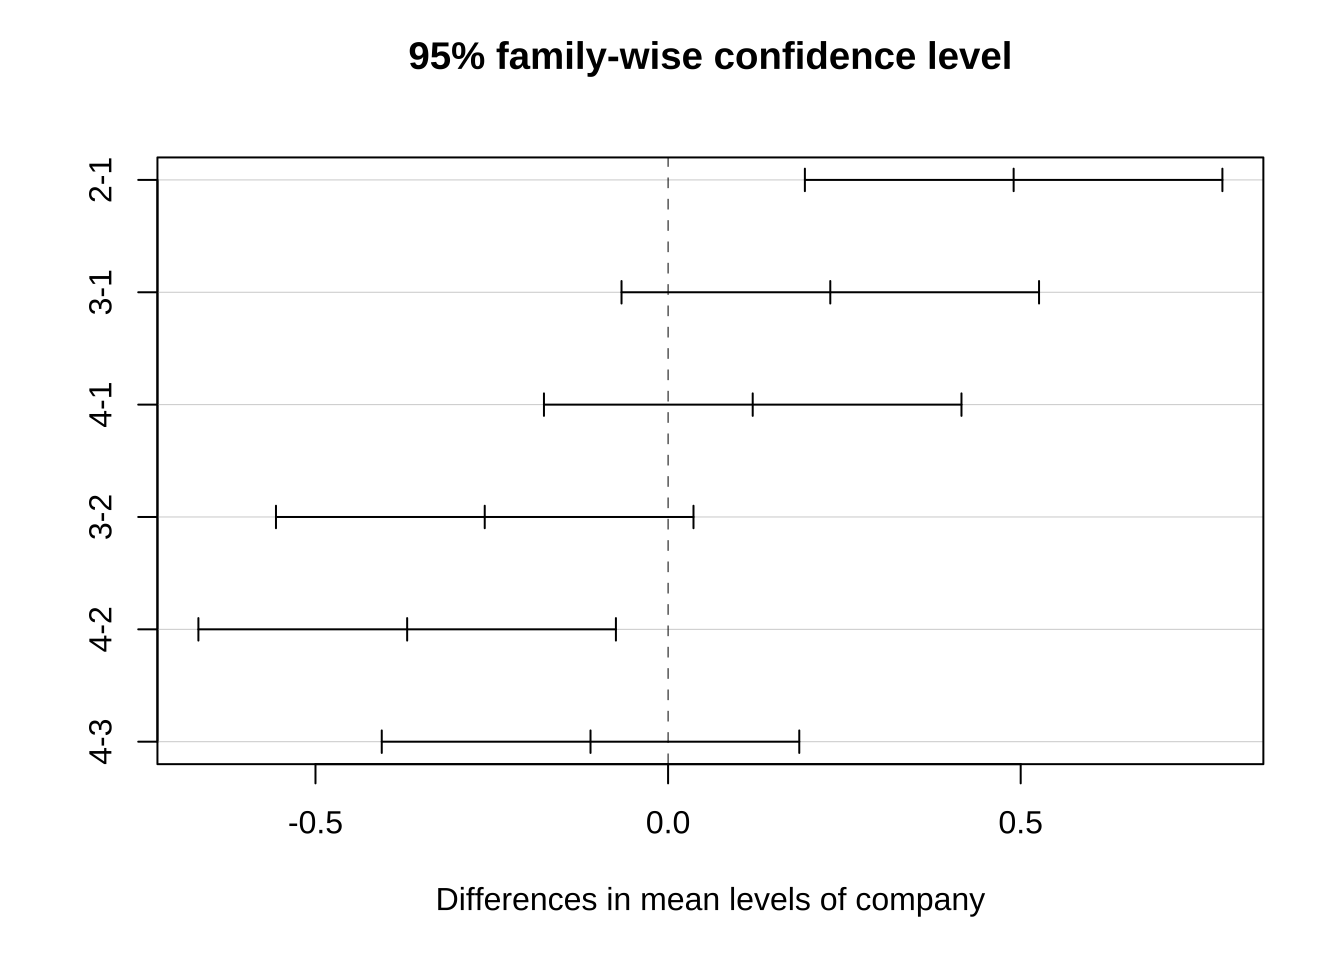
\includegraphics{qmd/lse_files/figure-pdf/unnamed-chunk-16-1.pdf}

잔차의 절대값보다 제곱한 양이 다루기가 쉬우므로(why?) 평균 모형과 회귀
모형의 적합도를 비교하는 양으로서 다음과 같은 각각의 모형에서 나온
두개의 잔차제곱합을 생각할 수 있다.

먼저 평균 모형은 예측에 사용할 변수가 없는 경우로서 이때의 잔차는 각
관측값에 대한 예측값이 관측값의 평균이다 . 이러한 경우 잔차는 관측값
자체가 가지고 있는 변동으로 생각할 수 있다. 이러한 평균모형에서의 잔차
또는 관측값이 가지고 있는 변동을 총제곱합(Total Sum of Squares ;
\(SST\))이다

\[
\begin{align}
\sum_{i=1}^n r^2_{0i} & = \sum_{i=1}^n (y_i -\bar y)^2 \\
  & =  \text{ Residual Sum of Squares from mean model }  \\
   & = \text{ Variation of response variables} \\
   & = \text{ Total Sum of Squares } \\
   & = SST
\end{align}
\]

이제 설명변수가 있는 회귀모형에서 예측치
\(\hat y_i=\hat \beta_0 + \hat \beta_1 x_i\)를 고려하면 이 경우의
잔차들의 제곱합은 회귀식의 잔차제곱합(Residual Sum of Squares;
\(SSE\))이라고 부르며 아래와 같이 정의한다.

\[
\begin{align}
\sum_{i=1}^n r_i^2 & = \sum_{i=1}^n (y_i -\hat \beta_0 - \hat \beta_1 x_i) \\
  & = \text{Residual Sum of Squares from linear regression model } \\
  & = \text{ Residual Sum of Squares } \\
  & = SSE 
\end{align}
\]

만약 회귀식에서 고려한 설명변수가 반응변수를 예측하는데 매우 적합하다면
회귀모형에서 구한 잔차들의 제곱합이 평균모형에서 구한 잔차들의
제곱합보다 작을 것이다. 이러한 차이를 비교하려면 두 제곱합 \(SST\) 와
\(SSE\)의 관계를 이해하는 것이 중요하다.

두 제곱합 \(SST\) 와 \(SSE\)의 관계를 보기 위하여 먼저 두 잔차 \(r^0_i\)
와 \(r_i\)의 차이를 비교해 보자

\[ r^0_i - r_i = (y_i - \bar y) - (y_i - \hat y_i) = \hat y_i - \bar y \]

위의 식에서 두 잔차의 차이 \(\hat y_i - \bar y\)는 예측값과 평균 간
차이로서 그 절댸값이 크면 회귀직선이 반응변수를 설명할 수 있는 능력이
크다는 것을 의미한다.

위의 식을 다시 쓰면 다음과 같다.

\[  (y_i - \bar y) = (y_i - \hat y_i) + (\hat y_i - \bar y) \]

즉, (평균모형의 잔차)=(회귀모형의 잔차))+(회귀모형의 설명부분)으로
분해되는 것으로 이해할 수 있다. 이 분해에서 회귀모형의 잔차가 작을수록
회귀 모형의 예측 능력, 즉 적합도가 커지는 것을 알 수 있다.

이제 총제곱합은 다음과 같이 분해할 수 있다.

\[
\begin{align}
 \sum^n_{i=1}(y_i - \bar y)^2 &=  \sum^n_{i=1}[(y_i-\hat y_i)+(\hat y_i - \bar y)]^2 \\
 &= \sum^n_{i=1}(y_i-\hat y_i)^2+\sum^n_{i=1}(\hat y_i - \bar y)^2
        + 2\sum^n_{i=1}(y_i-\hat y_i)(\hat y_i-\bar y)  \\
 &= \sum^n_{i=1}(y_i-\hat y_i)^2+\sum^n_{i=1}(\hat y_i - \bar y)^2 + 0 \quad \text{(why?)}
\end{align}
\]

따라서 다음과 같은 제곱합의 분해를 얻게 된다.

\[ 
\sum^n_{i=1}(y_i - \bar y)^2 = \sum^n_{i=1}(y_i-\hat y_i)^2+\sum^n_{i=1}(\hat y_i - \bar y)^2
\] 여기서 모형제곱합(regression sum of square; SSR)를 다음과 같이
정의하면

\[  SSR = \sum^n_{i=1}(\hat y_i-\bar y_i)^2 \]

총제곱합은 잔차제곱합 과 모형제곱합으로 분해된다.

\begin{equation}\phantomsection\label{eq-ssqdecomp}{
 SST = SSE + SSR 
}\end{equation}

관측값들이 보여주는 총 변동인 총제곱합(SST)에서 회귀모형으로 설명할 수
있는 변동, 즉 모형제곱합(SSR)이 차지하는 비율을 결정계수(coefficient of
determination)라 하며 \(R^2\)으로 표현한다.

\[ 
R^2 = \frac{SSR}{SST} =  1 -\frac{SSE}{SST}  =1- \frac{\sum^n_{i=1}(y_i-\hat y_i)^2}{ \sum^n_{i=1}(y_i - \bar y)^2} 
\]

위에서 정의된 \(R^2\) 는 평균 모형의 잔차제곱합 \(SST\)과 회귀모형의
잔차제곱합 \(SSE\)의 비율로 정의되는 것으로 해석할 수 있다. 즉,

\[  
R^2 = 1 -\frac{SSE}{SST} =1 -\frac{\text{Residual SS from regression model}}{\text{Residual SS from mean model}} 
\]

결정계수의 정의를 보면 회귀모형의 잔차제곱합(\(SSE\))가 평균 모형의
잔차제곱합(\(SST\))에 대하여 \textbf{상대적으로} 작아질수록 결정계수가
커진다. 결정계수 \(R^2\)는 언제나 0 이상 1 이하의 값을 갖는다.
회귀모형이 데이터에 아주 잘 적합되면 결정계수의 값은 1 에 가깝게 된다.

\section{중회귀 모형}\label{uxc911uxd68cuxadc0-uxbaa8uxd615}

일반적으로 회귀모형에서 반응변수의 수는 하나인 경우가 많지만 설명변수의
수는 여러 개인 경우가 많다. 이런 경우 중회귀 모형(multiple linear
regression)은 다음과 같이 표현할 수 있고, \(p-\)개의 설명변수가 있다고
가정하고 \((x_1, x_2, \cdots, x_{p-})\) 표본의 크기 \(n\)인 자료가
얻어지면 선형회귀식을 행렬로 다음과 같이 표현할 수 있다.

\begin{equation}\phantomsection\label{eq-multireg1}{
y_i = \beta_0 + \beta_1 x_{i1} + \beta_2 x_{i2} + \cdots + \beta_{p} x_{i,p} +  e_i = \pmb x^t_i \pmb \beta +  e_i 
}\end{equation}

위의 식을 다시 표현하면 다음과 같이 쓸 수 있다.

\[ 
y_i  = \pmb x^t_i \pmb \beta  + e_i  =
\begin{bmatrix}
1 & x_{i1} & x_{i2} & \cdots & x_{i,p}
\end{bmatrix}
\begin{bmatrix}
\beta_{0} \\
\beta_{1} \\
\beta_{2} \\
\vdots \\
\beta_{p}
\end{bmatrix}
+ e_i
\]

이제 \(n\)개의 관측치 \(y_1,y_2, \dots, y_n\) 으로 이루어진 관측값 벡터
\(\pmb y\)를 고려하면 n개의 관측치에 대한 회귀식을 행렬식으로 다음과
같이 표현할 수 있다.

\[ 
\begin{bmatrix}
y_{1} \\
y_{2} \\
\vdots \\
y_{n}
\end{bmatrix} =
\begin{bmatrix}
1 & x_{11} & \cdots & x_{1,p} \\
1 & x_{21} & \cdots & x_{2,p} \\
\vdots & \vdots & \vdots & \vdots \\
1 & x_{n1} & \cdots & x_{n,p}
\end{bmatrix}
\begin{bmatrix}
\beta_{0} \\
\beta_{1} \\
\vdots \\
\beta_{p}
\end{bmatrix}
+
\begin{bmatrix}
 e_{1} \\
 e_{2} \\
\vdots \\
 e_{n}
\end{bmatrix}
\]

위의 식을 간단히 행렬식으로 표시하면 다음과 같다.

\begin{equation}\phantomsection\label{eq-multireg2}{
\pmb y = \pmb X \pmb \beta + \pmb e
}\end{equation}

위의 행렬식에서 각 벡터와 행렬의 차원은 다음과 같다.

\begin{itemize}
\tightlist
\item
  \(\pmb y\): \(n \times 1\)
\item
  \(\pmb X\): \(n \times (p+1)\)
\item
  \(\pmb \beta\): \((p+1) \times 1\)
\item
  \(\pmb e\): \(n \times 1\)
\end{itemize}

여기서 회귀분석의 오차항 \(e_i\)은 서로 설명이고 동일한 분산을 갖는다.
즉, 오차항은 다음의 분포를 따른다.

\[ \pmb e  \sim (\pmb 0,\sigma^2 \pmb I_n) \]

따라서 관측값 벡터 \(\pmb y\)의 평균은 다음과 같고

\begin{equation}\phantomsection\label{eq-multiregmean}{
E(\pmb y|\pmb X) = E(\pmb X \pmb \beta+\pmb e)= \pmb X \pmb \beta + E(\pmb e) = \pmb X \pmb \beta
}\end{equation}

\(\pmb y\)의 분산은 아래와 같이 주어진다.

\begin{equation}\phantomsection\label{eq-multiregvar}{
 V( \pmb y| \pmb X) = E[( \pmb y -  \pmb X \pmb \beta)( \pmb y -  \pmb X \pmb \beta)^t] = E( \pmb  e   \pmb  e^t) = \sigma^2 \pmb I_n
}\end{equation}

여기서 오차항이 정규분포를 따른다면

\[ \pmb  e   \sim N(\pmb 0,\sigma^2 \pmb I_n) \]

관측값 벡터 \(\pmb y\) 또한 정규분포를 따른다

\[  \pmb y \sim N( \pmb X \pmb \beta, \sigma^2 \pmb I_n) \]

\subsection{최소제곱추정}\label{uxcd5cuxc18cuxc81cuxacf1uxcd94uxc815}

이제 중회귀모형 식~\ref{eq-multireg2} 에서 회귀계수벡터 \(\pmb \beta\)의
추정량을 구하기 위하여 최소제곱법을 적용해보자.

\begin{equation}\phantomsection\label{eq-rsq2}{
\min_{\pmb \beta} \sum_{i=1}^n (y_i -  \pmb x_i^t \pmb \beta )^2 = \min_{\pmb \beta } ( \pmb y -  \pmb X \pmb \beta )^t( \pmb y -  \pmb X \pmb \beta ) 
}\end{equation}

\subsubsection{방법 1}\label{uxbc29uxbc95-1}

\(\hat {\pmb \beta}\)는 잔차의 제곱합 식~\ref{eq-rsq2} 을 최소로 하는
최소제곱 추정량이다. 잔차의 제곱합을 \(S( \pmb \beta)\)이라고 하면

\begin{equation}\phantomsection\label{eq-rsq3}{
\begin{align} 
S( \pmb \beta ) & =  ( \pmb y -  \pmb X \pmb \beta)^t( \pmb y -  \pmb X \pmb \beta ) \notag \\
  & = \pmb y^t \pmb y - \pmb y^t \pmb X \pmb \beta - \pmb \beta^t \pmb X^t \pmb y
    + \pmb \beta^t \pmb X^t \pmb X \pmb \beta \notag \\
  & = \pmb y^t \pmb y -2  \pmb \beta^t \pmb X^t \pmb y
    + \pmb \beta^t \pmb X^t \pmb X \pmb \beta 
\end{align}
}\end{equation}

여기서 \(S( \pmb \beta)\)를 최소로 하는 회귀계수벡터의 값을 구하기
위하여 \(S( \pmb \beta)\)를 회귀계수벡터 \(\pmb \beta\)로 미분한후
\(\pmb 0\) 으로 놓고 선형 방정식을 풀어야 한다.

벡터미분을 이용하면

\[
\begin{align}
 \pardifftwo{ S( {\pmb \beta})}{\pmb \beta} & = 
 \pardifftwo{}{\pmb \beta} (\pmb y^t \pmb y -2  \pmb \beta^t \pmb X^t \pmb y
    + \pmb \beta^t \pmb X^t \pmb X \pmb \beta) \\
 & = \pmb 0 -2 \pmb X^t \pmb y + 2 \pmb X^t \pmb X \pmb \beta \\
 & =\pmb 0
\end{align}
\]

최소제곱 추정량을 구하기 위한 정규방정식은 다음과 같이 쓸 수 있다.

\begin{equation}\phantomsection\label{eq-lsequation}{
\pmb X^t \pmb X \pmb \beta =  \pmb X^t \pmb y
}\end{equation}

방정식 식~\ref{eq-lsequation} 를 정규방정식(normal equation)이라고 한다.
만약 \(\pmb X^t \pmb X\)가 정칙행렬일 경우 최소제곱법에 의한 회귀계수
추정량 \(\hat {\pmb \beta}\) 다음과 같다.

\begin{equation}\phantomsection\label{eq-lsestimator}{
\hat {\pmb \beta} = ( \pmb X^t \pmb X)^{-1} \pmb X^t \pmb y
}\end{equation}

예측값 벡터 \(\hat {\pmb y}\) 는 \(E(\pmb y | \pmb X)\)의 추정치로서
다음과 같다.

\[ \hat E(\pmb y | \pmb X)= \hat {\pmb y} = \pmb X \hat {\pmb \beta} = \pmb  X(\pmb X^t \pmb X)^{-1} \pmb X^t y \]

만약 \(\pmb X^t \pmb X\)가 정칙행렬이 아닐 경우 최소제곱법에 의한
회귀계수 추정량 \(\hat {\pmb \beta}\)은 \(\pmb X^t \pmb X\)의 일반화
역행렬 \((\pmb X^t \pmb X)^-\)를 이용하여 다음과 같이 구한다. 이 경우
일반화 역행렬이 유일하지 않기 때문에 회귀계수 추정량도 유일하지 않다.

\[
  \hat {\pmb \beta} = ( \pmb X^t \pmb X)^{-} \pmb X^t \pmb y
\]

\subsubsection{방법 2}\label{uxbc29uxbc95-2}

식~\ref{eq-rsq2} 에서 나오는 오차벡터를 정의하고
\(\pmb e = (\pmb y - \pmb X \pmb \beta)\) 오차벡터를 모수벡터
\(\pmb \beta\)로 미분하면 다음과 같은 결과를 얻는다.

\[ 
\pardifftwo{\pmb e}{\pmb \beta} = \pardifftwo{ (\pmb y - \pmb X \pmb \beta)}{ \pmb \beta} =
- \pardifftwo{ \pmb X \pmb \beta}{ \pmb \beta} \equiv
- \pardifftwo{\pmb \beta^t \pmb X^t }{\pmb \beta} = -\pmb X^t 
\]

이제 오차제곱합 \(S( {\pmb \beta})=\pmb e^t \pmb e\) 를 모수벡터로
미분하면 이차형식의 미분공식과 합성함수 미분공식을 차례로 적용하면 된다.

\[  
\pardifftwo{ S( {\pmb \beta})}{\pmb \beta}=\pardifftwo{\pmb e^t \pmb e}{\pmb \beta} =  \pardifftwo{\pmb e }{\pmb \beta} \pardifftwo{\pmb e^t  \pmb e}{\pmb e} = -\pmb X^t \left( 2 \pmb e \right ) = -2 \pmb X^t (\pmb y - \pmb X \pmb \beta)  
\]

위의 방정식을 \(\pmb 0\)으로 놓으면 최소제곱 추정량 (열)벡터를 구한다.

\[ 
\pmb X^t \pmb y - \pmb X^t  \pmb X \pmb \beta = \pmb 0 \quad \rightarrow \quad
\hat{\pmb \beta}  = (\pmb X^t  \pmb X)^{-1} \pmb X^t  \pmb y 
\] \#\# 최소제곱 추정량의 분포

회귀식을 추정하기 위한 회귀계수 추정값인 \(\hat {\pmb \beta}\)의 분포를
알아보기 위해서 우선 선형추정량을 보면 다음과 같다.

\[ \hat {\pmb \beta}  = (\pmb X^t\pmb X)^{-1}\pmb X' \pmb y \equiv  \pmb M \pmb y \]
따라서 최소제곱 추정량은 관측값들의 선형 변환이다. 회귀계수 추정값
\(\hat {\pmb \beta}\)의 기대값은

\[
\begin{align}
 E( \hat {\pmb \beta}  ) &= E( \pmb M \pmb y) = E(( \pmb X^t \pmb X)^{-1} \pmb X' \pmb y) \\
 &= ( \pmb X^t \pmb X)^{-1} \pmb X'E( \pmb y) \\
 &= ( \pmb X^t \pmb X)^{-1} \pmb X^t \pmb X \pmb \beta \\
  &= \pmb \beta
\end{align}
\]

따라서 최소제곱 추정량 \(\hat {\pmb \beta}\)는 \(\pmb \beta\)의
불편추정량이다. 최소제곱 추정량 \(\hat {\pmb \beta}\)의 공분산 행렬을
전개해보면

\[
\begin{align}
 Var( \hat {\pmb \beta} ) &= Var(( \pmb X^t \pmb X)^{-1} \pmb X^t \pmb y) \\
&= ( \pmb X^t \pmb X)^{-1} \pmb X^t ~ Var( \pmb y) ~ \pmb X ( \pmb X^t \pmb X)^{-1} \\
&=( \pmb X^t \pmb X)^{-1} \pmb X^t[\sigma^2  \pmb I_n] \pmb X( \pmb X^t \pmb X)^{-1} \\
&= \sigma^2( \pmb X^t \pmb X)^{-1} \pmb X^t \pmb X( \pmb X^t \pmb X)^{-1} \\
&= \sigma^2( \pmb X^t \pmb X)^{-1} \\
\end{align}
\]

위에서 최소제곱 추정량의 평균과 공분산을 구할 때에는 정규성 가정이
필요하지않다. 만일 \(\pmb y\)가 정규분포를 따른다면 \(\pmb y\)의
선형변환으로부터 얻어진 \(\hat {\pmb \beta}\)의 분포는 정규분포이며
다음과 같다.

\[  \hat {\pmb \beta}  \sim N \left (\pmb \beta, \sigma^2( \pmb X^t \pmb X)^{-1} \right ) \]

\section{가우스-마코브
정리}\label{uxac00uxc6b0uxc2a4-uxb9c8uxcf54uxbe0c-uxc815uxb9ac}

\begin{theorem}[가우스-마코브
정리]\protect\hypertarget{thm-line}{}\label{thm-line}

선형회귀모형 \(\pmb y =  \pmb X  \pmb \beta +  \pmb e\)에서
\(E( \pmb e)=0, Var( \pmb e)=\sigma^2 \pmb I\)이 성립하면 최소제곱
추정량

\[ \hat{\pmb \beta}=(\pmb X^t \pmb X)^{-1} \pmb X^t \pmb y\]

는 \(\pmb \beta\)의 최소분산 선형 불편추정량이다.

\end{theorem}

위의 정리를 가우스-마코브 정리 (Gauss-Markov Theorem)라고 하며 이는
회귀계수 \(\pmb \beta\)의 모든 선형 불편 추정량들 중에 최소제곱 추정량
\(\hat {\pmb \beta}=(\pmb X^t \pmb X)^{-1} \pmb X^t \pmb y\)이 가장 작은
분산을 가짐을 뜻한다 (Best Linear Unbiased Estimator; BLUE).

가우스-마코브 정리를 정확하게 표현하면
\(E(\pmb L \pmb y) = \pmb \beta\)를 만족하는 모든 \(n \times n\) 차원의
행렬 \(\pmb L\)과 임의의 벡터 \(\pmb c\)에 대하여 다음이 성립한다.

\[ V(\pmb c^t \hat {\pmb \beta}) \le V(\pmb c^t \pmb L \pmb y)  \]

이제 가우스-마코브 정리를 증명해보자. 관측벡터 \(\pmb y\)에 대한 임의의
선형 추정량 \(\pmb \beta^* = \pmb L \pmb y\)를 생각해보면 다시 다음의
형태로 표시할 수 있다.

\[  
\pmb \beta^* =  \pmb L  \pmb y = (\pmb M + \pmb L -\pmb M ) \pmb y = ( \pmb M +  \pmb A)  \pmb y 
\]

여기서 \(\pmb M = ( \pmb X^t \pmb X)^{-1} \pmb X^t\) 이고
\(\pmb A= \pmb L- \pmb M\) 이다. 임의의 선형 추정량 \(\pmb \beta^*\)가
불편 추정량일 조건을 구해보자

\[
\begin{align}
 E( \pmb \beta^*) & = E[( \pmb M+ \pmb A) \pmb y] \\
            & = ( \pmb M+ \pmb A)E( \pmb y) \\
            & = ( \pmb M+ \pmb A)X \pmb \beta \\
            & = ( \pmb X^t  \pmb X)^{-1} \pmb X^t  \pmb X  \pmb \beta +  \pmb A  \pmb X  \pmb \beta \\
            & =  \pmb \beta+AX \pmb \beta\\
\end{align}
\]

여기서 불편추정량이 되기 위해서는 \(E( \pmb \beta^*)= \pmb \beta\)
조건을 만족 해야되며 따라서 \(\pmb A \pmb X=0\)이되어야한다 (이 조건은
\(\pmb A=0\)를 의미하는 것은 아니다).

이제 최소분산을 가지기 위해서 \(\pmb A \pmb X=0\)을 만족하는 행렬
\(\pmb A\)중에서 \(Var( \pmb \beta^*)\)을 최소로하는 행렬 \(\pmb A\)를
구해야 한다. \(\pmb \beta^*\)의 공분산 행렬은 \(AX=0\)이므로

\[
\begin{align}
 V( \pmb \beta^*) & = ( \pmb M+ \pmb A)V( \pmb y)( \pmb M+ \pmb A)^t\\
            & = ( \pmb M+ \pmb A)\sigma^2 I_n( \pmb M+ \pmb A)^t\\
            & = \sigma^2 ( \pmb M \pmb M^t+ \pmb A \pmb M^t+ \pmb M  \pmb A^t+ \pmb A  \pmb A^t)\\
            & = \sigma^2 [ ( \pmb X^t  \pmb X)^{-1}  \pmb X^t  \pmb X( \pmb X^t \pmb X)^{-1} + \pmb A  \pmb X ( \pmb X^t  \pmb X)^{-1}+( \pmb X^t  \pmb X)^{-1} \pmb X^t  \pmb A^t+  \pmb A  \pmb A^t ]\\
            & = \sigma^2[( \pmb X^t  \pmb X)^{-1} +  \pmb A  \pmb A^t ]  \\
            & = V( \hat {\pmb \beta} ) + \sigma^2 \pmb A \pmb A^t\\
\end{align}
\]

이제 임의의 벡터 \(\pmb c\)에 대하여

\[
\begin{align}
 V( \pmb c^t \pmb \beta^*)  & = \pmb c^t V (\pmb \beta^*) \pmb c \\
   & =  \pmb c^t V( \hat {\pmb \beta} ) \pmb c + \sigma^2 \pmb c^t \pmb A \pmb A^t \pmb c \\
    & =  V( \pmb c^t  \hat {\pmb \beta} ) + \sigma^2 \pmb c^t \pmb A \pmb A^t \pmb c 
\end{align}
\]

다음이 성립하므로

\[ \pmb c^t \pmb A \pmb A^t \pmb c = \pmb u^t \pmb u = \sum_{i=1}^n u_i^2 \ge 0 \]

임의의 벡터 \(\pmb c\)에 대하여

\[ V( \pmb c^t \pmb \beta^*) \ge  V( \pmb c^t  \hat {\pmb \beta} ) \]

이제 \(V( \pmb c^t \pmb \beta^*)\) 이
\(V( \pmb c^t \hat {\pmb \beta} )\)과 같으려면 다음 조건이 성립해야 하며

\[ \pmb u = \pmb c^t \pmb A = \pmb 0 \]

임의의 모든 벡터 \(\pmb c\)에 대해서 위의 조건 성립해야 하므로 이는
\(\pmb A = \pmb 0\) 이 성립해야 한다. 또한 이조건은
\(\pmb A \pmb X=0\)도 만족 시켜준다. 따라서 \(\pmb \beta\)의 최소분산
선형 불편추정량은 최소제곱법으로 구한 추정량이다.

여기서 주의할 점은 가우스-마코브 정리에서 관측값 \(\pmb y\)에 대한
가정은 평균과 공분산의 가정만 주어졌으며 \(\pmb y\)의 분포에 대한 가정이
없다. 참고로 만약에 \(\pmb y\)가 정규분포를 따른다면 최소제곱 추정량은
최소분산 불편추정량이다.

\section{최대가능도
추정}\label{uxcd5cuxb300uxac00uxb2a5uxb3c4-uxcd94uxc815}

관측값 벡터 \(\pmb y\) 가 다음과 같이 선형모형이며 정규분포를 따른다고
가정하자.

\begin{equation}\phantomsection\label{eq-normallm}{
\pmb y \sim N( \pmb X \pmb \beta, \sigma^2 \pmb I_n) 
}\end{equation}

선형모형 식~\ref{eq-normallm} 에 대한 가능도 함수는 다음과 같이
주어진다.

\[
\begin{align}
 L_n( \pmb \theta ;  \pmb y) & = L( \pmb \beta,\sigma^2|  \pmb y) \\
   & = \prod^n_{i=1} f(y_i)\\
   & = \prod^n_{i=1}(2 \pi \sigma^2)^{-\frac{1}{2}} \exp \left [-\frac{1}{2\sigma^2} (y_i- {\pmb x}_i^t \pmb \beta)^2 \right ] \\
   & = (2\pi\sigma^2)^{-\frac{n}{2}} \exp \left [ -\frac{1}{2\sigma^2}( \pmb y- \pmb  X  \pmb \beta)^t( \pmb y- \pmb X  \pmb \beta) \right ]
\end{align}
\]

또한 분산에 대한 모수를 \(\tau=\sigma^2\) 과 같이 쓰면 로그 가능도함수는
다음과 같다.

\[
\begin{align}
\ell_n( \pmb \theta; \pmb y) & = -\frac{n}{2} \log (2 \pi)-\frac{n}{2} \log \sigma^2 -\frac { ( \pmb y- \pmb X  \pmb \beta)^t (\pmb  y- \pmb X  \pmb \beta) }{2\sigma^2} \\ 
   &= -\frac{n}{2} \log (2 \pi)-\frac{n}{2} \log \tau -\frac { ( \pmb y- \pmb X  \pmb \beta)^t ( \pmb y- \pmb X  \pmb \beta) }{2\tau}  
\end{align}
\]

이제 로그가능도함수로부터 구할 수 있는 스코어함수
\(s( \pmb \theta;\pmb y)\) 와 그에 대한 관측 피셔정보
\(J_n( \pmb \theta; \pmb y)\) 은 다음과 같이 주어진다.

\[
\begin{align}
s( \pmb \theta;  \pmb y) & =  \pardifftwo{}{ \pmb \theta}\ell_n( \pmb \theta;  \pmb y ) \\
  & =  \begin{bmatrix}
    \pardifftwo{}{ \pmb  \beta}\ell_n( \pmb \theta;  \pmb y ) \\
    \pardifftwo{}{\tau}\ell_n( \pmb \theta;  \pmb y ) 
  \end{bmatrix} \\
  & = 
  \begin{bmatrix}
     \pmb X^t ( \pmb y- \pmb X  \pmb \beta)/\tau \\
    -\frac{n}{2\tau} +\frac { ( \pmb y- \pmb X  \pmb \beta)^t ( \pmb y- \pmb X  \pmb \beta) }{2\tau^2} 
  \end{bmatrix} \\
 J_n( \pmb \theta;  \pmb y) & =  -\pardifftwo{}{ \pmb \theta}{ {\pmb \theta}^t}\ell_n( \pmb \theta;\pmb y ) \\
  & = 
  - \begin{bmatrix}
    \pardifftwo{}{\pmb \beta}{ {\pmb \beta}^t}\ell_n( \pmb \theta;\pmb y ) & \pardifftwo{}{ \pmb \beta}{\tau^t}\ell_n( \pmb \theta;\pmb y )  \\
    \pardifftwo{}{\tau}{ {\pmb \beta}^t}\ell_n( \pmb \theta;\pmb y )  & \pardifftwo{}{\tau}{\tau}\ell_n( \pmb \theta; \pmb y ) 
  \end{bmatrix} \\
   & = 
  \begin{bmatrix}
      {\pmb X}^t  \pmb X /\tau &  - {\pmb X}^t ( \pmb y- \pmb X  \pmb \beta)/\tau^2   \\
    - {\pmb X}^t ( \pmb y- \pmb X  \pmb \beta)/\tau^2  &  - \frac{n}{2\tau^2} +\frac { ( \pmb y- \pmb X \pmb  \beta)^t ( \pmb y- \pmb X  \pmb \beta) }{\tau^3} 
  \end{bmatrix}
\end{align}
\]

이제 중회귀모형에서 회귀계수 \(\pmb \beta\)에 대한 최대가능도 추정량은
스코어함수로 부터 얻어진 방정식 \(s( \pmb \theta; y)= 0\) 으로부터
얻어지며 다음과 같은 형태를 가진다.

\[ \hat { \beta} = ( {\pmb X}^t  \pmb X)^{-1} {\pmb  X}^t  \pmb y \]

\[   \hat \sigma^2 = \hat \tau = ( \pmb y-\pmb  X  \hat {\pmb \beta})^t ( \pmb y- \pmb X  \hat {\pmb \beta})/n = \frac{SSE(\hat{\pmb  \beta})}{n} \]

여기서 유의할 점은 회귀계수 \(\pmb \beta\) 의 최대가능도 추정량은
최소제곱법으로 구한 추정량과 동일하다. 따라서 \(\hat {\pmb  \beta}\)은
최소분산 불편 추정량이다. 하지만 오차항의 분산 \(\sigma^2\) 에 대한
최대가능도 추정량은 불편추정량이 아니다.

\[ E(\hat \sigma^2)  = E \left [ ( \pmb y- \pmb X  {\hat {\pmb \beta}})^t ( \pmb y-\pmb  X  {\hat {\pmb \beta}})/n \right ] = E \left [ \frac{SSE}{n} \right ]  \ne \sigma^2 \]

참고로 오차항의 분산 \(\sigma^2\)에 대한 불편추정량은 \(SSE/(n-p)\)이다.
오차항의 분산에 대한 불편추정량은 다음 장에서 논의할 것이다.

최대가능도 추정량의 점근적 분포를 이용하면 다음과 같이 말할 수 있다.
오차항이 정규분포인 선형모형인 경우 아래의 분포는 점근분포가 아닌 정확한
분포이다.

\[ \hat { \pmb \theta}  \sim  N( \pmb \theta ,  I_n^{-1}( \pmb \theta)) \]

여기서

\[  I_n( \pmb \theta) = E[ J( \pmb \theta;  y)] =  
\begin{bmatrix}
      {\pmb X}^t \pmb X /\tau & 0   \\
    0  &   \frac{n}{2\tau^2} 
  \end{bmatrix}
\] 그리고 \[  I_n^{-1}( \pmb \theta) = 
\begin{bmatrix}
     \tau( {\pmb X}^t  \pmb X)^{-1}  & 0   \\
    0  &   \frac{2\tau^2}{n} 
  \end{bmatrix}
  = 
\begin{bmatrix}
     \sigma^2( {\pmb X}^t  \pmb X)^{-1}  & 0   \\
    0  &   \frac{2\sigma^4}{n} 
  \end{bmatrix}
\]

따라서 회귀계수 추정량 \(\hat { \beta}\)의 분포는 평균이 \(\pmb \beta\)
이고 공분산이 \(\sigma^2( {\pmb X}^t - \pmb X)^{-1}\) 인 정규분포를
따른다.

여기거 주목할 점은 가능도함수에 최대가능도추정량을 대입하면 그 값이
\(SSE(\hat { \beta})\)의 함수로 나타난다.

\begin{equation}\phantomsection\label{eq-likefull}{
\begin{align}
 L_n(\hat { \pmb \theta} ) & = L_n(\hat { \pmb \beta} ,\hat \sigma^2 ) \notag \\
 &=  (2\pi\hat \sigma^2)^{-\frac{n}{2}} \exp \left [-\frac{1}{2 \hat \sigma^2}( \pmb y- \pmb X \hat { \pmb \beta})^t( \pmb y- \pmb X \hat { \pmb \beta} ) \right ] \notag  \\
& = (2\pi\hat \sigma^2)^{-\frac{n}{2}} \exp \left [-\frac{n}{2} \right ]  \notag  \\
& = \left (2\pi \frac{SSE(\hat { \pmb \beta})}{n} \right )^{-\frac{n}{2}} \exp \left [-\frac{n}{2} \right ] 
\end{align} 
}\end{equation} 또한 가능도함수의 값은 다음과 같다.

\begin{equation}\phantomsection\label{eq-linregloglike}{
l_n(\hat { \pmb \theta} ) = l_n(\hat { \pmb \beta} ,\hat \sigma^2 ) 
= \text{constant}  - \frac{n}{2} \log \frac{SSE(\hat { \pmb \beta})}{n}
}\end{equation}

따라서 잔차제곱함 \(SSE(\hat { \pmb \beta})\) 작아지면 가능도함수는
커진다.

앞 절에서 언급한 평균 모형 식~\ref{eq-meanmodel} 에서 최대가능도 추정을
알아보자. 관측값 벡터는 다음과 같은 분포를 따른다.

\begin{equation}\phantomsection\label{eq-meanlm}{
\pmb y \sim N( \beta_0 \pmb 1 , \sigma^2 \pmb I_n) 
}\end{equation}

선형모형 식~\ref{eq-normallm} 에 대한 로그 가능도 함수는 다음과 같이
주어진다. 분산에 대한 모수를 \(\tau=\sigma^2\) 로 바꾸어 사용하면 모수
벡터는 \(\pmb \theta = (\beta_0, \tau)^t\)이다.

\[ 
\ell_n( \pmb \theta; \pmb y) = -\frac{n}{2} \log (2 \pi)-\frac{n}{2} \log \tau -\frac { ( \pmb y- \beta_0 \pmb 1  )^t ( \pmb y-  \beta_0 \pmb 1) }{2\tau}  
\]

두 개의 모수 \(\beta_0\)와 \(\tau\)에 대하여 미분하여 가능도 방정식을
구하면 다음과 같다.

\[
\begin{align}
s( \pmb \theta;  \pmb y) & =  \pardifftwo{}{ \pmb \theta}\ell_n( \pmb \theta;  \pmb y ) \\
  & =  \begin{bmatrix}
    \pardifftwo{}{ \beta_0}\ell_n( \pmb \theta;  \pmb y ) \\
    \pardifftwo{}{\tau}\ell_n( \pmb \theta;  \pmb y ) 
  \end{bmatrix} \\
  & = 
  \begin{bmatrix}
     \pmb 1^t ( \pmb y-  \beta_0 \pmb 1)/\tau \\
    -\frac{n}{2\tau} +\frac { ( \pmb y- \beta_0 \pmb 1))^t ( \pmb y- \beta_0 \pmb 1) }{2\tau^2} 
  \end{bmatrix} \\
  & = \pmb 0
\end{align}
\]

위의 방정식을 풀면 다음과 같은 최대가능도 추정량을 구할 수 있다.

\[
\hat \beta_0 = \bar y, \quad {\hat \sigma}^2 = \frac{\sum_{i=1}^n (y_i - \bar y)^2}{n} = \frac{SST}{n} 
\]

그리고 가능도함수에 최대가능도추정량을 대입하면 그 값이 다음과 같다.

\begin{equation}\phantomsection\label{eq-likemean}{
 L_n(\hat { \pmb \theta} )  = L_n(\hat { \beta_0} ,\hat \sigma^2 ) 
 = \left (2\pi \frac{SST}{n} \right )^{-\frac{n}{2}} \exp \left [-\frac{n}{2} \right ]
}\end{equation}

두 개의 모형, 즉 선형회귀모형 식~\ref{eq-normallm} 과 평균모형
식~\ref{eq-meanmodel} 의 가능도 함수의 비, 즉 식~\ref{eq-likefull} 과
식~\ref{eq-likemean} 의 비율을 구해보면 결정계수 \(R^2\)외의 관계를 볼
수 있다.

\[  
\frac{ L_n(\hat { \beta_0} ,\hat \sigma^2 )  }{L_n(\hat { \pmb \beta} ,\hat \sigma^2 ) }
= \left (2\pi \frac{SST}{n} \right )^{-\frac{n}{2}} / \left (2\pi \frac{SSE}{n} \right )^{-\frac{n}{2}} 
\propto  \left [ \frac{SSE}{SST} \right ]^{\frac{n}{2}} = \left [ 1-R^2 \right ]^{\frac{n}{2}}  
\]

\bookmarksetup{startatroot}

\chapter*{References}\label{references}
\addcontentsline{toc}{chapter}{References}

\markboth{References}{References}

\phantomsection\label{refs}
\begin{CSLReferences}{1}{0}
\bibitem[\citeproctext]{ref-kang2016you}
강근석, 와/과 유형조. 2016. \emph{{R}을 활용한 선형회귀분석}. 1st ed.
교우사. \url{https://github.com/regbook/regbook}.

\end{CSLReferences}

\cleardoublepage
\phantomsection
\addcontentsline{toc}{part}{Appendices}
\appendix

\chapter{행렬의 기초}\label{uxd589uxb82cuxc758-uxae30uxcd08}

이 장에서는 회귀분석의 이론 전개에 필요한 행렬 이론과 선형 대수의 기초에
대하여 알아볼 것이다.

\section{벡터와 행렬}\label{uxbca1uxd130uxc640-uxd589uxb82c}

다음 \(p\)-차원 벡터(vector) 또는 열벡터(column vector) \(\pmb a\) 는
\(p\)개의 원소 \(a_1, a_2, \dots, a_p\) 를 하나의 열(column)에 배치한
형태를 가진 개체이다.

\[
\pmb a = 
\begin{bmatrix}
a_1 \\
a_2 \\
\vdots \\
a_p 
\end{bmatrix}
\]

차원이 \(n \times p\) 인 행렬 \(\pmb A\) 는 다음과 같이 \(n\)개의 행과
\(p\) 개의 열에 원소 \(a_{ij}\)를 다음과 같이 배치한 형태를 가진다.

\[
\pmb A = 
\begin{bmatrix}
a_{11} & a_{12} & \dots & a_{1p} \\
a_{21} & a_{22} & \dots & a_{2p} \\
\vdots & \vdots &    & \dots \\
a_{n1} & a_{n2} & \dots & a_{np} 
\end{bmatrix}
\]

\section{두 행렬의 덧셈}\label{uxb450-uxd589uxb82cuxc758-uxb367uxc148}

두 행렬 \(\pmb A\) 와 \(\pmb B\) 를 더하는 규칙은 다음과 같다.

\begin{itemize}
\tightlist
\item
  두 행렬 \(\pmb A\) 와 \(\pmb B\) 는 행과 열의 갯수가 같아야 한다.
\item
  \(\pmb A + \pmb B = \pmb C\) 라고 하면, 덧셈의 결과로 만들어진 행렬
  \(\pmb C\)는 두 행렬과 같은 수의 행과 열을 가지면 각 원소는 다음과
  같다.
\end{itemize}

\[ \pmb A + \pmb B = \pmb C \quad \rightarrow \quad c_{ij} = a_{ij} + b_{ij} \]

\section{스칼라곱}\label{uxc2a4uxce7cuxb77cuxacf1}

임의의 실수 \(\lambda\) (스칼라)가 주어졌을 때, \(\lambda\) 와 행렬
\(\pmb A\)의 스칼라곱(scalar product) 는 행렬의 모든 원소에 \(\lambda\)
를 곱해준 행렬로 정의된다.

예를 들어 \(\lambda=2\), \(\pmb A \in \RR^{2\times 3}\) 인 경우

\[
\lambda \pmb A = 
2
\begin{bmatrix}
1 & 2 & 3 \\
-1 & 0 & 2
\end{bmatrix}
=
\begin{bmatrix}
2 & 4 & 6 \\
-2 & 0 & 4
\end{bmatrix}
\]

\section{벡터와 행렬의
곱셈}\label{uxbca1uxd130uxc640-uxd589uxb82cuxc758-uxacf1uxc148}

\(n \times p\) 인 행렬 \(\pmb A\) 와 \(p\)-차원 벡터(vector)
\(\pmb b\)는 다음과 같이 두 개의 서로 다른 형태로 나타낼 수 있다.

먼저 행렬과 벡터의 곱셈은 행렬 \(\pmb A\) 의 행벡터와 벡터 \(\pmb b\) 의
내적(inner product)로 나타낼 수 있다.

\[
\begin{align}
{\pmb A} {\pmb b} & = 
\begin{bmatrix}
a_{11} & a_{12} & \dots & a_{1p} \\
a_{21} & a_{22} & \dots & a_{2p} \\
\vdots & \vdots &    & \dots \\
a_{n1} & a_{n2} & \dots & a_{np} 
\end{bmatrix}
\begin{bmatrix}
b_1 \\
b_2 \\
\vdots \\
b_p 
\end{bmatrix} \\
& = 
\begin{bmatrix}
{\pmb r}^t_1 \\
{\pmb r}^t_2 \\
\vdots \\
{\pmb r}^t_n 
\end{bmatrix} 
\begin{bmatrix}
b_1 \\
b_2 \\
\vdots \\
b_p 
\end{bmatrix} 
\quad 
\text{ where }
{\pmb r}^t_i =
\begin{bmatrix}
a_{i1} & a_{i2} & \dots & a_{ip} 
\end{bmatrix}  \\
& = 
\begin{bmatrix}
{\pmb r}^t_1 {\pmb b} \\
{\pmb r}^t_2 {\pmb b} \\
\vdots \\
{\pmb r}^t_n {\pmb b}
\end{bmatrix}  
 = 
\begin{bmatrix}
\sum_{j=1}^p a_{1j} b_j \\
\sum_{j=1}^p a_{2j} b_j \\
\vdots \\
\sum_{j=1}^p a_{nj} b_j
\end{bmatrix} \\
& = 
\begin{bmatrix}
 <\pmb r_1, \pmb b>  \\
 <\pmb r_2, \pmb b> \\
\vdots \\
 <\pmb r_n, \pmb b>
\end{bmatrix}
\end{align}
\]

위에서 \(< \pmb a, \pmb b>\) 는 다음과 같은 두 벡터의 내적(inner
product)을 의미한다.

\[ < \pmb a, \pmb b> = {\pmb a}^t {\pmb b} = \sum_{i=1}^p a_i b_i \]

이제 행렬과 벡터의 곱셈을 행렬을 구성하는 열벡터들의 선형조합(linear
combination)으로 나타낼 수 있다.

\[
\begin{align}
{\pmb A} {\pmb b} & = 
\begin{bmatrix}
a_{11} & a_{12} & \dots & a_{1p} \\
a_{21} & a_{22} & \dots & a_{2p} \\
\vdots & \vdots &    & \dots \\
a_{n1} & a_{n2} & \dots & a_{np} 
\end{bmatrix}
\begin{bmatrix}
b_1 \\
b_2 \\
\vdots \\
b_p 
\end{bmatrix} \\
& = 
\begin{bmatrix}
{\pmb c}_1 & {\pmb c}_2 & \dots & {\pmb c}_p 
\end{bmatrix} 
\begin{bmatrix}
b_1 \\
b_2 \\
\vdots \\
b_p 
\end{bmatrix} 
\quad 
\text{ where }
{\pmb c}_j =
\begin{bmatrix}
a_{1j} \\
a_{2j} \\
\vdots \\
a_{nj} 
\end{bmatrix} \\
& =
b_1 
\begin{bmatrix}
a_{11} \\
a_{21} \\
\vdots \\
a_{n1} 
\end{bmatrix} 
+ 
b_2 
\begin{bmatrix}
a_{12} \\
a_{22} \\
\vdots \\
a_{n2} 
\end{bmatrix} 
+ \cdots + 
b_p 
\begin{bmatrix}
a_{1p} \\
a_{2p} \\
\vdots \\
a_{np} 
\end{bmatrix}  \\
& =
b_1 {\pmb c}_1 + b_2 {\pmb c}_2 + \cdots + b_p {\pmb c}_p \\
\end{align}
\]

\section{행렬의 전치}\label{uxd589uxb82cuxc758-uxc804uxce58}

\(\pmb A^t\)는 행렬의 전치(transpose)를 나타낸다.

\section{행렬의 곱셈}\label{uxd589uxb82cuxc758-uxacf1uxc148}

먼저 두 행렬 \(\pmb A\) 와 \(\pmb B\) 의 곱셈

\[ \pmb A \times \pmb B \equiv \pmb A \pmb B \]

을 정의하려면 다음과 같은 조건이 만족되어야 한다.

\begin{itemize}
\tightlist
\item
  행렬 \(\pmb A\) 의 열의 갯수와 행렬 \(\pmb B\) 의 행의 갯수가 같아야
  한다
\end{itemize}

따라서 두 행렬의 곱셈은 순서를 바꾸면 정의 자체가 안될 수 있다.

이제 두 행렬 \(\pmb A \in \RR^{m \times n}\) 와
\(\pmb B \in \RR^{n \times k}\)의 곱셈은 다음과 같이 정의된다.

\[ \pmb A \pmb B =  \pmb C\]

행렬 \(\pmb C\) 는 \(m\) 개의 행과 \(k\)개의 열로 구성된
행렬이며(\(\pmb C \in \RR^{m \times k}\)) 각 원소 \(c_{ij}\)는 다음과
같이 정의된다.

\[  c_{ij} = \sum_{l=1}^n a_{il} b_{lk}, \quad i=1,2,\dots,m; j=1,2,\dots,k \]

먼저 간단한 예제로 다음과 같은 두 개의 행렬의 곱을 생각해 보자.

\[
\pmb A \pmb B =
\begin{bmatrix}
1 & 2 \\
3 & 4 
\end{bmatrix}
\begin{bmatrix}
0 & 1 \\
-1 & 2
\end{bmatrix}
=
\begin{bmatrix}
(1)(0) + (2)(-1) & (1)(1) + (2)(2) \\
(3)(0) + (4)(-1) & (3)(1) + (4)(2)
\end{bmatrix}
=
\begin{bmatrix}
-2 & 5 \\
-4 & 11
\end{bmatrix}
\]

곱하는 순서를 바꾸어 계산해 보자.

\[
\pmb B \pmb A =
\begin{bmatrix}
0 & 1 \\
-1 & 2
\end{bmatrix}
\begin{bmatrix}
1 & 2 \\
3 & 4 
\end{bmatrix}
=
\begin{bmatrix}
(0)(1) + (1)(3) & (0)(2) + (1)(4) \\
(-1)(1) + (2)(3) & (-1)(2) + (2)(4)
\end{bmatrix}
=
\begin{bmatrix}
3 & 4 \\
5 & 6
\end{bmatrix}
\]

위 두 결과를 보면 행렬의 곱셈에서는 교환법칙이 성립하지 않음을 알 수
있다.

이제 차원이 다른 두 행렬의 곱셈을 살펴보자.

\[
\pmb A =
\begin{bmatrix}
1 & 2 & 3\\
3 & 2 & 1
\end{bmatrix},
\quad
\pmb B =
\begin{bmatrix}
0 & 2 \\
1 & -1 \\
0 & 1
\end{bmatrix}
\]

두 행렬의 곱셈은 다음과 같이 계산할 수 있다.

\[
\pmb A \pmb B =
\begin{bmatrix}
1 & 2 & 3\\
3 & 2 & 1
\end{bmatrix}
\begin{bmatrix}
0 & 2 \\
1 & -1 \\
0 & 1
\end{bmatrix}
=
\begin{bmatrix}
2 & 3 \\
2 & 5
\end{bmatrix}
\]

두 행렬의 곱하는 순서를 바꾸면 차원이 전혀 다른 행렬이 얻어진다.

\[
\pmb B \pmb A =
\begin{bmatrix}
0 & 2 \\
1 & -1 \\
0 & 1
\end{bmatrix}
\begin{bmatrix}
1 & 2 & 3\\
3 & 2 & 1
\end{bmatrix}
=
\begin{bmatrix}
6 & 4 & 2 \\
-2 & 0 & 2 \\
3 & 2 & 1
\end{bmatrix}
\]

\textbf{행렬의 곱셈은 교환법칙이 성립하지 않는다.}

\begin{equation}\phantomsection\label{eq-product-not}{  \pmb A \pmb B \ne  \pmb B \pmb A}\end{equation}

\begin{tcolorbox}[enhanced jigsaw, colback=white, title=\textcolor{quarto-callout-caution-color}{\faFire}\hspace{0.5em}{주의}, colbacktitle=quarto-callout-caution-color!10!white, toprule=.15mm, breakable, bottomtitle=1mm, left=2mm, colframe=quarto-callout-caution-color-frame, leftrule=.75mm, coltitle=black, toptitle=1mm, titlerule=0mm, arc=.35mm, opacityback=0, opacitybacktitle=0.6, rightrule=.15mm, bottomrule=.15mm]

\textbf{교환법칙이 성립하지 않는다}는 의미는 식~\ref{eq-product-not} 이
언제나 성립한다는 의미는 아니다. 아래와 같이 특별한 경우 교환법칙이
성립하는 경우도 있다.

\[
\begin{bmatrix}
1 & 2 \\
1 & 3 
\end{bmatrix}
\begin{bmatrix}
1 & 0 \\
0 & 1 
\end{bmatrix}
=
\begin{bmatrix}
1 & 2 \\
1 & 3 
\end{bmatrix}
=
\begin{bmatrix}
1 & 0 \\
0 & 1 
\end{bmatrix}
\begin{bmatrix}
1 & 2 \\
1 & 3 
\end{bmatrix}
\]

\end{tcolorbox}

\begin{itemize}
\tightlist
\item
  행렬의 곱셈은 결합법칙과 배분법칙은 성립한다.
\end{itemize}

\[ (\pmb A \pmb B) \pmb C = \pmb A (\pmb B \pmb C) \]

\[ (\pmb A + \pmb B) \pmb C = \pmb A \pmb C +  \pmb B \pmb C \]

\section{단위벡터와
항등행렬}\label{uxb2e8uxc704uxbca1uxd130uxc640-uxd56duxb4f1uxd589uxb82c}

\(i\)번째 단위벡터 \(\pmb e_i\)를 정의하자. 단위벡터 \(\pmb e_i\)는
\(n\)- 차원 벡터로서 \(i\)번째 원소만 1이고 나머지는 0인 벡터이다.

\[ \pmb e_i = 
\begin{bmatrix}
0 \\
0 \\
\vdots \\ 
0 \\  
1 \\
0 \\
\vdots \\
0 
\end{bmatrix}
\]

즉 \(n\)-차원 항등행렬 \(\pmb I\)는 n개의 단위벡터들을 모아놓은 것이다.

\[  \pmb I = [ \pmb e_1 ~~ \pmb e_2 ~~ \dots ~~ \pmb e_n ] \]

\section{대각합}\label{uxb300uxac01uxd569}

\(\pmb A = \{ a_{ij} \}\)를 \(n \times n\) 정방행렬(square matrix)인
경우, 행렬의 대각합(trace)을 \(tr(\pmb A)\)로 표시한다.

\[ tr(\pmb A) = \sum_{i=1}^n a_{ii} \]

행렬의 곱셈은 일반적으로 교환법칙이 성립하지 않지만 대각합의 연산은
교환법칙이 성립한다.

\[  tr(\pmb A \pmb B)  = tr( \pmb B \pmb A) \]

두 행렬의 덧셈(뺄셈)에 대한 대각합에 대한 성질들은 다음과 같다.

\[ tr( {\pmb A} \pm {\pmb B}) = tr({\pmb A}) \pm tr({\pmb B}) \]

\section{행렬식}\label{uxd589uxb82cuxc2dd}

\(\pmb A\)의 행렬식(determinant)을 \(det(\pmb A)=|\pmb A|\)로 표기한다.

만약 행렬 \(\pmb A\)가 대각행렬(diagonal matrix)이면 \(|\pmb A|\)는
행렬의 대각원소의 곱이다 (\(| \pmb A| =\prod a_{ii}\)).

두 행렬의 곱의 행렬식은 각 행렬의 행렬식의 곱이다.

\[ |\pmb A \pmb B | = | \pmb A| |\pmb B| \]

행렬식에 대한 유용한 공식들은 다음과 같다.

\begin{itemize}
\tightlist
\item
  \(|{\pmb A}^t| = |{\pmb A}|\)
\item
  \(|c {\pmb A}| = c^n |{\pmb A}|\)
\end{itemize}

만약 행렬 \(\pmb A\)가 다음과 같은 분할행렬(partitioned matrix) 의
형태를 가지면

\[ 
\pmb A =
\begin{bmatrix}
{\pmb A}_{11} & {\pmb A}_{12} \\
{\pmb 0} & {\pmb A}_{22}
\end{bmatrix}
\]

행렬 \(\pmb A\)의 행렬식은 다음과 같이 주어진다.

\[ |{\pmb A}| = |{\pmb A}_{11}| |{\pmb A}_{22} | \]

\chapter{고유값과 고유벡터}\label{eigen-01}

\begin{tcolorbox}[enhanced jigsaw, colback=white, title=\textcolor{quarto-callout-caution-color}{\faFire}\hspace{0.5em}{주의}, colbacktitle=quarto-callout-caution-color!10!white, toprule=.15mm, breakable, bottomtitle=1mm, left=2mm, colframe=quarto-callout-caution-color-frame, leftrule=.75mm, coltitle=black, toptitle=1mm, titlerule=0mm, arc=.35mm, opacityback=0, opacitybacktitle=0.6, rightrule=.15mm, bottomrule=.15mm]

고유값과 고유벡터는 정방행렬(square matrix)에 대해서만 정의된다.

\end{tcolorbox}

\section{특성다항식}\label{uxd2b9uxc131uxb2e4uxd56duxc2dd}

특성다항식(Characteristic polynomial)은 다음과 같이 정의된다

실수 \(\lambda \in \mathbb{R}\) 와 정방행렬(square matrix)
\(\boldsymbol{A} \in \mathbb{R}^{n \times n}\) 에 대하여

\begin{equation}\phantomsection\label{eq-char-poly}{
\begin{aligned}
p_{\boldsymbol{A}}(\lambda) & :=\operatorname{det}(\boldsymbol{A}-\lambda \boldsymbol{I}) \\
& =c_0+c_1 \lambda+c_2 \lambda^2+\cdots+c_{n-1} \lambda^{n-1}+(-1)^n \lambda^n,
\end{aligned}
}\end{equation}

\section{고유값과
고유벡터}\label{uxace0uxc720uxac12uxacfc-uxace0uxc720uxbca1uxd130}

\subsection{정의}\label{uxc815uxc758}

\(n\)-차원 정방행렬 \(\pmb A\) 이 있을 때, 다음 식을 만족하는
\(\lambda\) 와 벡터 \(\pmb x\)가 존재하면 \(\lambda\) 를 행렬 \(\pmb A\)
의 고유값(eigenvalue), \(\pmb x\) 를 행렬 \(\pmb A\) 의
고유벡터(eigenvector)라고 한다 (부교재 definition 4.6)

\[ \pmb A \pmb x = \lambda \pmb x \]

\begin{itemize}
\tightlist
\item
  고유벡터는 유일하지 않다. 즉, 벡터 \(\pmb x\) 가 고유벡터이면
  \(c \pmb x\) 도 고유벡터이다.
\end{itemize}

\[ \pmb A (c \pmb x) = c \pmb A \pmb x = c \lambda \pmb x = \lambda (c \pmb x) \]

\subsection{계산}\label{uxacc4uxc0b0}

다음 3개의 문장은 동치이다

\begin{itemize}
\tightlist
\item
  \(\lambda\) 는 행렬 \(\pmb A\) 의 고유값이다.
\item
  방정식 \((\pmb A - \lambda \pmb I)\pmb x = \pmb 0\) 은 영벡터이외의
  해를 가진다(nontrivial solution)
\item
  \(\lambda\) 는 행렬 \(\pmb A - \lambda \pmb I\) 의 행렬식이 0이다.
\end{itemize}

\begin{equation}\phantomsection\label{eq-char-poly2}{ \operatorname{det}(\pmb A - \lambda \pmb I) = 0 }\end{equation}

\begin{itemize}
\item
  \(\lambda\) 는 행렬 \(\pmb A - \lambda \pmb I\) 의 rank가 \(n\) 보다
  작다.
\item
  Theorem 4.8 에 의하면 위에서 행렬식이 0 인 방정식
  식~\ref{eq-char-poly2} 을 푸는 것은 식~\ref{eq-char-poly} 의 이 0 을
  푸는 것과 동일하다는 것이다.
\end{itemize}

\subsection{중복도와
고유공간}\label{uxc911uxbcf5uxb3c4uxc640-uxace0uxc720uxacf5uxac04}

부교재의 Definition 4.9, 4.10, 4.11 에 대한 내용입니다.

\begin{itemize}
\item
  대수적 중복도(algebraic multiplicity) 는 특성다항식
  식~\ref{eq-char-poly} 이 0인 방정식을 푸는 경우 다항식에서 고유값이
  중근(multiple root)의 해로 나타나는 차수를 의미한다.
\item
  기하적 중복도(geometric multiplicity) 는 고유값에 대응하는 고유벡터들
  중 선형독립인 고유벡터들의 최대 개수를 의미한다.
\item
  고유 공간(eigenspace)은 고유값에 대응하는 고유벡터들이 생성하는
  벡터공간을 의미한다.
\end{itemize}

\begin{center}\rule{0.5\linewidth}{0.5pt}\end{center}

\begin{exercise}[]\protect\hypertarget{exr-Example-20-1}{}\label{exr-Example-20-1}

3차원 행렬 \(\pmb A\) 가 다음과 같을 때

\[\pmb A=\left[\begin{array}{ccc}0 & 0 & -2 \\ 1 & 2 & 1 \\ 1 & 0 & 3\end{array}\right]\]

행렬 \(\pmb A\)의 특성다항식은 다음과 같다.

\[
\operatorname{det}(\lambda \pmb I -\pmb A)= 
\left|\begin{array}{ccc}
\lambda & 0 & 2 \\
-1 & \lambda-2 & -1 \\
-1 & 0 & \lambda-3
\end{array}\right|=(\lambda-1)(\lambda-2)^2
\] 참고로 특성방정식을 푸는 경우, 방정식
\(\operatorname{det}(\pmb A - \lambda \pmb I)=0\) 이나
\(\operatorname{det}(\lambda \pmb I -\pmb A)= 0\) 중 어느 것을 사용해도
상관없다.

첫번째 고유값은 \(\lambda_1=1\) 이다. 고유벡터를 구하기 위해서는 다음과
같은 방정식을 풀면 된다.

\[ (\lambda_1 \pmb I -\pmb A )\pmb x = \pmb 0  \]

위의 방정식을 풀면

\[
(\lambda_1 \pmb I -\pmb A )\pmb x= (\pmb I -\pmb A )\pmb x
=
\begin{bmatrix}
1 & 0 & 2 \\
-1 & -1 & -1 \\
-1 & 0 & -2
\end{bmatrix}
\begin{bmatrix}
x_1 \\
x_2 \\
x_3 \\
\end{bmatrix}
=
\begin{bmatrix}
0 \\
0 \\
0 \\
\end{bmatrix}
\]

아래와 같이 간단히 할 수 있으며

\[ x_1 = -2x_3, \quad x_2 = x_3 \] 다음과 같은 고유값과 고유벡터를 얻을
수 있다.

\[ \lambda_1=1 \quad \rightarrow \quad  x_1=\begin{bmatrix}-2 \\ 1 \\ 1\end{bmatrix} \]

\textbf{첫번째 고유값은 \(\lambda_1=1\) 이며 대수적 중복도는 1이고
기하적 중복도도 1이다.} 이 경우 고유공간 \(E_1\) 은 한 개의 고유벡터
\(\pmb x_1\) 이 생성하는 부분공간을 의미한다.

\[
E_1 = \text{span}\left\{\begin{bmatrix}-2 \\ 1 \\ 1\end{bmatrix} \right\}
\]

다음으로 두번째 고유값에 대한 방정식
\((\lambda_2 \pmb I -\pmb A )\pmb x = \pmb 0\) 을 풀면 다음과 같다.

\[
(\lambda_2 \pmb I -\pmb A )\pmb x= (2\pmb I -\pmb A )\pmb x =
\begin{bmatrix}
2 & 0 & 2 \\
-1 & 0 & -1 \\
-1 & 0 & -1
\end{bmatrix}
\begin{bmatrix}
x_1 \\
x_2 \\
x_3 \\
\end{bmatrix}
=
\begin{bmatrix}
0 \\
0 \\
0 \\
\end{bmatrix}
\]

이 방정식은 아래와 같이 간단히 할 수 있으며

\[ x_1 = -x_3 \] 다음과 같은 두 개의 고유벡터를 얻을 수 있다.

\[ 
\lambda_2=2\quad \rightarrow \quad  x_2=\begin{bmatrix}-1 \\ 0 \\ 1\end{bmatrix} 
\quad x_3=\begin{bmatrix}0 \\ 1 \\ 0\end{bmatrix} 
\]

위에서 \textbf{두번째 고유값은 \(\lambda_2=2\) 이며 대수적 중복도는
2이다.} 또한 \textbf{선형독립인 2개의 고유벡터를 구할 수 있으므로 기하적
중복도는 2이다.}

이 경우 \(E_2\) 는 두 개의 고유벡터 \(\pmb x_1, \pmb x_2\) 가 생성하는
부분공간을 의미한다.

\[
E_2 = \text{span}\left\{\begin{bmatrix}-1 \\ 0 \\ 1\end{bmatrix}, \begin{bmatrix}0 \\ 1 \\ 0\end{bmatrix}\right\}
\]

\(\blacksquare\)

\end{exercise}

\begin{center}\rule{0.5\linewidth}{0.5pt}\end{center}

이제 대수적 중복도와 기하적 중복도가 다른 경우에 대한 예제를 들어보자.

\begin{center}\rule{0.5\linewidth}{0.5pt}\end{center}

\begin{exercise}[]\protect\hypertarget{exr-Example-20-2}{}\label{exr-Example-20-2}

3차원 행렬 \(\pmb A\) 가 다음과 같을 때

\[\pmb A=\left[\begin{array}{ccc}1 & 0 & 2 \\ -1 & 1 & 3 \\ 0 & 0 & 2\end{array}\right]\]

행렬 \(\pmb A\)의 특성다항식은 다음과 같다.

\[
\operatorname{det}(\lambda \pmb I -\pmb A)= 
\left|\begin{array}{ccc}
\lambda-1 & 0 & -2 \\
1 & \lambda-1 & -3  \\
0 & 0 & \lambda-2
\end{array}\right|=(\lambda-1)^2(\lambda-2)
\] 첫번째 고유값은 \(\lambda_1=1\) 이다. 고유벡터를 구하기 위해서는
다음과 같은 방정식을 풀면 된다.

\[ (\lambda_1 \pmb I -\pmb A )\pmb x = \pmb 0  \]

위의 방정식을 풀면

\[
(\lambda_1 \pmb I -\pmb A )\pmb x= (\pmb I -\pmb A )\pmb x =
\begin{bmatrix}
0 & 0 & -2 \\
1 & 0 & -3 \\
0 & 0 & -1
\end{bmatrix}
\begin{bmatrix}
x_1 \\
x_2 \\
x_3 \\
\end{bmatrix}
=
\begin{bmatrix}
0 \\
0 \\
0 \\
\end{bmatrix}
\]

아래와 같이 간단히 할 수 있으며

\[ \quad x_1 = x_3 =0 \] 다음과 같은 하나의 고유벡터를 얻을 수 있다.

\[ \lambda_1=1 \quad \rightarrow \quad  x_1=\begin{bmatrix} 0 \\ 1 \\ 0 \end{bmatrix} \]

\textbf{첫번째 고유값은 \(\lambda_1=1\) 이며 대수적 중복도는 2이지만
기하적 중복도는 1이다.} 이 경우 고유공간 \(E_1\) 은 한 개의 고유벡터
\(\pmb x_1\) 이 생성하는 부분공간을 의미한다.

\[
E_1 = \text{span}\left\{\begin{bmatrix}0 \\ 1 \\ 0\end{bmatrix} \right\}
\]

다음으로 두번째 고유값에 대한 방정식
\((\lambda_2 \pmb I -\pmb A )\pmb x = \pmb 0\) 을 풀면 다음과 같다.

\[
(\lambda_2 \pmb I -\pmb A )\pmb x= (2\pmb I -\pmb A )\pmb x = 
\begin{bmatrix}
1 & 0 & 2 \\
1 & 1 & -3 \\
0 & 0 & 0
\end{bmatrix}
\begin{bmatrix}
x_1 \\
x_2 \\
x_3 \\
\end{bmatrix}
=
\begin{bmatrix}
0 \\
0 \\
0 \\
\end{bmatrix}
\]

이 방정식은 아래와 같이 간단히 할 수 있으며

\[ x_1 = -2x_3, \quad x_2=5x_3  \] 다음과 같은 한 개의 고유벡터를 얻을
수 있다.

\[ 
\lambda_2=2\quad \rightarrow \quad  x_2=\begin{bmatrix}-2 \\ 5 \\ 1\end{bmatrix} 
\]

위에서 \textbf{두번째 고유값은 \(\lambda_2=2\) 이며 대수적 중복도는
1이다.} 또한 \textbf{선형독립인 1개의 고유벡터를 구할 수 있으므로 기하적
중복도는 1이다.}

이 경우 \(E_2\) 는 한 개의 고유벡터 \(\pmb x_2\) 가 생성하는 부분공간을
의미한다.

\[
E_2 = \text{span}\left\{\begin{bmatrix}-2\\ 5 \\ 1\end{bmatrix}\right\}
\]

\(\blacksquare\)

\end{exercise}

\begin{center}\rule{0.5\linewidth}{0.5pt}\end{center}

\chapter{벡터 미분}\label{vector-cal-01}

\section{용어}\label{uxc6a9uxc5b4}

\begin{itemize}
\tightlist
\item
  vector differential: 벡터 미분
\item
  partial derivative: 편미분
\item
  gradient: 그레디언트
\item
  Jacobian: 야코비안, 자코비안
\end{itemize}

\section{벡터 미분의
표기법}\label{uxbca1uxd130-uxbbf8uxbd84uxc758-uxd45cuxae30uxbc95}

이제 다변량함수(multivariate function), \(f: \RR^n \rightarrow \RR^m\)에
대한 미분을 생각해보자.

먼저 간단한 예제를 고려해 보자. 두 열벡터

\[
\pmb x=
\begin{bmatrix}
x_1 \\ 
x_2
\end{bmatrix}
\in \RR_2, \quad 
\pmb y=
\begin{bmatrix}
y_1 \\
y_2 \\ 
y_3 
\end{bmatrix} \in \RR^3
\]

를 고려하고 다음과 같은 함수로 두 벡터의 관계가 정의된다고 하자.

\begin{equation}\phantomsection\label{eq-vec-cal-xy}{ 
y_1 = x_1^2 + x_2, \quad y_2= \exp (x_1) + 3 x_2, \quad y_3 = \sin(x_1) + x_2^3 
}\end{equation}

위의 관계를 함수 관계 \(\pmb f: \RR^2 \rightarrow \RR^3\) 로 나타내보면

\[ 
 \pmb f(\pmb x) = 
\begin{bmatrix} f_1(\pmb x) \\ f_2 (\pmb x) \\ f_3(\pmb x) \end{bmatrix} = 
\begin{bmatrix} x_1^2 + x_2 \\ \exp (x_1) + 3 x_2 \\ \sin(x_1) + x_2^3 \end{bmatrix} =
\begin{bmatrix} y_1 \\ y_2 \\ y_3 \end{bmatrix} = \pmb y
\]

이러한 경우 다변량 함수 \(\pmb f\)를 벡터 \(\pmb x\)로 미분하려면, 즉
미분 표기법을 이용하려면 편미분을 한 결과를 행렬의 형태를 정해야한다.

\[  \pardifftwo{ \pmb f}{\pmb x} = (n \times m)-\text{matrix} \quad \text{ or }  \quad (m \times n)-\text{matrix}? \]

일단 각각의 편미분 \(\pardifftwo{f_i}{x_j}\)를 구해야 하며 이는 scalar
미분으로 쉽게 구해진다.

\begin{equation}\phantomsection\label{eq-par_deriv}{
\begin{aligned}
\pardifftwo{  f_1}{ x_1} & = 2x_1, & \quad \pardifftwo{  f_2}{ x_1} & = \exp(x_1), & \quad
\pardifftwo{  f_3}{ x_1} & = \cos(x_1) \\
\pardifftwo{  f_1}{ x_2} & = 1,    & \quad \pardifftwo{  f_2}{ x_1} & = 3,         & \quad
\pardifftwo{  f_3}{ x_1} & = 3 x_2^2 \\
\end{aligned}
}\end{equation}

이제 이제 편미분값들을 행렬의 형태로 정리해보자. 편미분을 행렬에 배치할
떄 다음과 같은 규칙을 사용할 것이다.

\begin{itemize}
\tightlist
\item
  행렬의 행은 \(\pmb x\)의 차원 \(n\) 과 같다.
\item
  행렬의 열은 \(\pmb f\)의 차원 \(m\) 과 같다.
\end{itemize}

위와 같이 편미분을 배치하는 벡타 미분 표기법을 분모 표기법 (denominator
layout)이라고 한다.

\begin{tcolorbox}[enhanced jigsaw, colback=white, title=\textcolor{quarto-callout-note-color}{\faInfo}\hspace{0.5em}{분모 표기법}, colbacktitle=quarto-callout-note-color!10!white, toprule=.15mm, breakable, bottomtitle=1mm, left=2mm, colframe=quarto-callout-note-color-frame, leftrule=.75mm, coltitle=black, toptitle=1mm, titlerule=0mm, arc=.35mm, opacityback=0, opacitybacktitle=0.6, rightrule=.15mm, bottomrule=.15mm]

\[ 
\pmb J = \nabla_x \pmb x =\pardifftwo{ \pmb f}{\pmb x}  \equiv \pardifftwo{ \pmb f^t}{\pmb x}
\underset{def}{\equiv} \begin{bmatrix}
\pardifftwo{  f_1}{ x_1} &  \pardifftwo{  f_2}{ x_1} &  \pardifftwo{  f_3}{ x_1}  \\
\pardifftwo{  f_1}{ x_2} &  \pardifftwo{  f_2}{ x_2}  &  \pardifftwo{  f_3}{ x_2} 
\end{bmatrix}
=  \begin{bmatrix}
2x_1 &  \exp(x_1)  &  \cos(x_1)   \\
1 &  3  &  3x_2^2
\end{bmatrix}
\] \(\pmb J\)는 야코비안 행렬(Jacobian matrix)이라고 부른다.

\end{tcolorbox}

이제 이러한 분자표기법의 특별한 결과를 알아보자

\begin{itemize}
\item
  \(f: \RR^n \rightarrow \RR^1\) 인 경우

  \(f: \RR^n \rightarrow \RR^1\) 인 경우 벡터미분 결과를
  \textbf{그레디언트(gradient)}라고 부르며 다음과 같이 표기된다.
\end{itemize}

\[ 
\nabla_x f = \pardifftwo{ f}{\pmb x} = 
\begin{bmatrix} 
\pardifftwo{ f}{x_1} \\
\pardifftwo{ f}{x_2} \\
\vdots \\ 
\pardifftwo{ f}{x_n} 
\end{bmatrix} 
\]

\begin{itemize}
\tightlist
\item
  \(f: \RR^1 \rightarrow \RR^m\) 인 경우
\end{itemize}

\[ 
\pardifftwo{\pmb f}{x} = 
\begin{bmatrix} 
\pardifftwo{ f_1}{x} \\
\pardifftwo{ f_2}{x} \\
\vdots \\
\pardifftwo{ f_m}{x} 
\end{bmatrix} 
\]

참고로 식~\ref{eq-vec-cal-xy} 에서 정의한 함수 관계를 두 벡터 \(\pmb x\)
와 \(\pmb y\) 의 사상관계로 보면

\[ \pmb f : \pmb x \mapsto \pmb y \] 다음과 같이 그레디언트 벡터를
표기할 수 있다.

\[  \pardifftwo{ \pmb f}{\pmb x} = \pardifftwo{ \pmb y}{\pmb x}
=
\begin{bmatrix}
\pardifftwo{  y_1}{ x_1} &  \pardifftwo{  y_2}{ x_1} &  \pardifftwo{  y_3}{ x_1}  \\
\pardifftwo{  y_1}{ x_2} &  \pardifftwo{  y_2}{ x_2}  &  \pardifftwo{  y_3}{ x_2} 
\end{bmatrix}
\]

\section{함성함수의
미분법}\label{uxd568uxc131uxd568uxc218uxc758-uxbbf8uxbd84uxbc95}

이제 합성함수의 미분법(chain rule)에 대하여 알아보자.

두 개의 함수

\[
\pmb g :\RR^n \mapsto \RR^m, \quad \pmb f :\RR^m \mapsto \RR^p
\] 가 있을 때, \(\pmb f\)와 \(\pmb g\)의 합성함수 \(\pmb h\)는 다음과
같이 정의된다.

\[ \pmb h( \pmb x) = \pmb f( \pmb g( \pmb x)) = \pmb f \circ \pmb g\]
즉,

\[ 
\pmb h : \RR^n \mapsto \RR^m \mapsto \RR^p
\]

이러한 합성함수의 미분은 다음과 같이 계산된다.

\begin{equation}\phantomsection\label{eq-vec-chain-01}{
\pardifftwo{ \pmb h}{\pmb x} = \pardifftwo{ \pmb f \circ \pmb g}{\pmb x} = \pardifftwo{ \pmb g}{\pmb x} \pardifftwo{ \pmb f}{\pmb g}
}\end{equation}

식~\ref{eq-vec-chain-01} 에서 \(\pardifftwo{ \pmb f}{\pmb g}\)는
\(m \times p\) Jacovian 벡터이고

\[ 
\pardifftwo{ \pmb f}{\pmb g} 
\begin{bmatrix}
\pardifftwo{  f_1}{ g_1} &  \pardifftwo{  f_2}{ g_1} & \cdots &  \pardifftwo{  f_p}{ g_1} \\
\pardifftwo{  f_1}{ g_2} &  \pardifftwo{  f_2}{ g_2} & \cdots &  \pardifftwo{  f_p}{ g_2} \\
\vdots & \vdots & \ddots & \vdots \\
\pardifftwo{  f_1}{ g_m} &  \pardifftwo{  f_2}{ g_m} & \cdots &  \pardifftwo{  f_p}{ g_m} \\
\end{bmatrix}
=(m \times p)
\]

\(\pardifftwo{ \pmb g}{\pmb x}\)는 \(n \times m\) Jacovian 벡터이다

\[
\pardifftwo{ \pmb g}{\pmb x} =
\begin{bmatrix}
\pardifftwo{  g_1}{ x_1} &  \pardifftwo{  g_2}{ x_1} & \cdots &  \pardifftwo{  g_m}{ x_1} \\
\pardifftwo{  g_1}{ x_2} &  \pardifftwo{  g_2}{ x_2} & \cdots &  \pardifftwo{  g_m}{ x_2} \\
\vdots & \vdots & \ddots & \vdots \\
\pardifftwo{  g_1}{ x_n} &  \pardifftwo{  g_2}{ x_n} & \cdots &  \pardifftwo{  g_m}{ x_n} \\
\end{bmatrix}
= (n \times m)
\]

함성함수의 미분 공식을 차원으로 나타내면 다음과 같다.

\[
\underset{ n \times p} {\pardifftwo{ \pmb h}{\pmb x}} = \underset{ n \times m} {\pardifftwo{ \pmb g}{\pmb x}} \underset{ m \times p} {\pardifftwo{ \pmb f}{\pmb g}}
\]

\section{두 벡터 내적의
미분}\label{uxb450-uxbca1uxd130-uxb0b4uxc801uxc758-uxbbf8uxbd84}

\subsection{상수벡터와 변수벡터의
내적}\label{uxc0c1uxc218uxbca1uxd130uxc640-uxbcc0uxc218uxbca1uxd130uxc758-uxb0b4uxc801}

먼저 상수 벡터 \(\pmb a\)와 변수 벡터 \(\pmb x\)의 내적의 미분을 생각해
보자.

참고로 다음과 같이 두 벡터의 내적은 스칼라이다.

\[ \pmb a^t \pmb x = \pmb x^t \pmb a = a_1 x_1 + a_2x_2 + \dots + a_n x_n \]

따라서 그레이디언트를 구하는 방법과 같이 결과는 열벡터로 표기된다.

\[
\pardifftwo{ \pmb a^t \pmb x}{\pmb x} = \pardifftwo{ \pmb x^t \pmb a}{\pmb x} = \pmb a =
\begin{bmatrix}
a_1 \\ 
a_2\\ 
\vdots \\
 a_n
\end{bmatrix}
\]

위의 식에서 상수벡터 \(\pmb a\)는 가 전치로 앞에 나타나는 표현
\(\pmb x^t \pmb a\) 를 사용하면 결과 벡터 \(\pmb a\)가 열벡터로 그대로
나타나지므로 \textbf{내적의 미분 표기}로 사용할 것이다.

\begin{equation}\phantomsection\label{eq-vec-diff}{ 
\pardifftwo{ \pmb x^t \pmb a}{\pmb x} =  \pardifftwo{  \pmb x^t}{\pmb x} \pmb a =\pmb I  \pmb a = \pmb a 
}\end{equation}

\subsection{상수벡터와 함수벡터의
내적}\label{uxc0c1uxc218uxbca1uxd130uxc640-uxd568uxc218uxbca1uxd130uxc758-uxb0b4uxc801}

더 나아가서 상수 벡터 \(\pmb a\)와 함수 벡터 \(\pmb f\)의 내적의 미분도
식~\ref{eq-vec-diff} 을 표시하는 동일한 논리로 다음과 같이 표기할 수
있다.

\begin{equation}\phantomsection\label{eq-vec-diff-0}{ 
\pardifftwo{ \pmb f^t \pmb a}{\pmb x} =  \pardifftwo{  \pmb f^t}{\pmb x} \pmb a
}\end{equation}

참고로 식~\ref{eq-vec-diff-0} 에서 \(\pardifftwo{  \pmb f}{\pmb x}\)는
행벡터가 아닌 행렬로 나타날 수 있다.

\subsection{함수벡터와 함수벡터의
내적}\label{uxd568uxc218uxbca1uxd130uxc640-uxd568uxc218uxbca1uxd130uxc758-uxb0b4uxc801}

이제 다음과 같이 같은 공간으로 사상되는 두 함수 \(\pmb f\) 와 \(\pmb g\)
의 내적을 생각해 보자.

\[ \pmb f : \RR^n \mapsto \RR^m, \quad \pmb g : \RR^n \mapsto \RR^m\]

두 함수의 내적을 미분하는 경우 곱셉 법칙을 적용하여야 하는데 행렬의
곱셉에서는 교환법칙이 성립되지 않으므로 순서에 주의해야 한다.

내적 \(\pmb f^t \pmb g\) 를 각각 따로 미분해야 하는데 각 벡터에 대해
따로 미분을 실행해 보자

\begin{itemize}
\tightlist
\item
  \(\pmb f\) 를 미분하는 경우 \(\pmb g\) 는 상수 벡터 \(\pmb a\) 로
  취급한다. 그리고 식~\ref{eq-vec-diff-0} 를 적용한다.
\end{itemize}

\begin{equation}\phantomsection\label{eq-vec-diff-1}{
\pardifftwo{ \pmb f^t \pmb g}{\pmb x} = \pardifftwo{ \pmb f^t \pmb a}{\pmb x} = 
=  \pardifftwo{ \pmb f^t}{\pmb x} \pmb a=
\pardifftwo{ \pmb f}{\pmb x} \pmb g
}\end{equation}

\begin{itemize}
\tightlist
\item
  \(\pmb g\) 를 미분하는 경우 \(\pmb f\) 는 상수 벡터 \(\pmb a\) 로
  취급한다. 그리고 식~\ref{eq-vec-diff-0} 를 적용한다.
\end{itemize}

\begin{equation}\phantomsection\label{eq-vec-diff-2}{
\pardifftwo{ \pmb f^t \pmb g}{\pmb x} = \pardifftwo{ \pmb a^t \pmb g}{\pmb x} = 
\pardifftwo{ \pmb g^t \pmb a}{\pmb x} = 
 \pardifftwo{ \pmb g^t}{\pmb x}  \pmb a =
 \pardifftwo{ \pmb g}{\pmb x} \pmb f 
}\end{equation}

이제 위의 두 결과 식~\ref{eq-vec-diff-1} 과 식~\ref{eq-vec-diff-2} 를
합치면 다음과 같은 최종적인 결과를 얻을 수 있다.

\begin{equation}\phantomsection\label{eq-vec-diff-prod}{
\pardifftwo{ \pmb f^t \pmb g}{\pmb x} =  \pardifftwo{ \pmb f}{\pmb x} \pmb g +  \pardifftwo{ \pmb g}{\pmb x} \pmb f
}\end{equation}

\section{벡터 미분의
응용}\label{uxbca1uxd130-uxbbf8uxbd84uxc758-uxc751uxc6a9}

\subsection{선형사상의
미분상}\label{uxc120uxd615uxc0acuxc0c1uxc758-uxbbf8uxbd84uxc0c1}

이제 앞에서 배운 벡터의 미분을 이용하여 유용한 응용 공식을 유도해보자.

먼저 선형변환 \(\pmb y = \pmb A \pmb x\) 를 생각해 보자. 이때
(\(M \times N\))-\(\pmb A\)는 상수 행렬이다. 이때 \(\pmb y\)를
\(\pmb x\)로 미분하면 다음과 같다.

먼저 행렬 \(\pmb A\)의 \(i\) 번째 행을 \(\pmb a_i^t\)라고 하면

\[
\pmb A = \begin{bmatrix}
A_{11} & A_{12} & \dots & A_{1N} \\
A_{21} & A_{22} & \dots & A_{2N} \\
\vdots & \vdots & \ddots & \vdots \\
A_{M1} & A_{M2} & \dots & A_{MN} \\
\end{bmatrix}=
\begin{bmatrix}
\pmb a_1^t  \\
\pmb a_2^t  \\
\vdots \\
\pmb a_M^t  \\
\end{bmatrix}
\]

선형변환 \(\pmb f(\pmb x) = \pmb A \pmb x\) 로 정의하면 다음과 같이
나타낼 수 있다.

\[
\pmb A \pmb x=
\begin{bmatrix}
\pmb a_1^t \pmb x \\
\pmb a_2^t \pmb x \\
\vdots \\
\pmb a_M^t \pmb x \\
\end{bmatrix} =
\begin{bmatrix}
f_1(\pmb x) \\
f_2(\pmb x) \\
\vdots \\
f_M(\pmb x) \\
\end{bmatrix} 
= \pmb f(\pmb x) 
\]

따라서

\[
\pardifftwo{\pmb A \pmb x}{\pmb x}   = \pardifftwo{\pmb f (\pmb x)}{\pmb x} =
\begin{bmatrix}
\pardifftwo{f_1}{x_1} & \pardifftwo{f_2}{x_1} & \dots & \pardifftwo{f_M}{x_1} \\
\pardifftwo{f_1}{x_2} & \pardifftwo{f_2}{x_2} & \dots & \pardifftwo{f_M}{x_2} \\
\vdots & \vdots & \ddots & \vdots \\
\pardifftwo{f_1}{x_N} & \pardifftwo{f_2}{x_N} & \dots & \pardifftwo{f_M}{x_N} \\
\end{bmatrix} =
\begin{bmatrix}
A_{11} & A_{21} & \dots & A_{M1} \\
A_{12} & A_{22} & \dots & A_{M2} \\
\vdots & \vdots & \ddots & \vdots \\
A_{1N} & A_{2N} & \dots & A_{MN} \\
\end{bmatrix} = \pmb A^t
\] 따라서 선형사상의 미분은 선형변환 행렬의 전치이다.

\begin{equation}\phantomsection\label{eq-vec-diff-linear}{ \pardifftwo{\pmb A \pmb x}{\pmb x}  = \pmb A^t }\end{equation}

\chapter{벡터공간}\label{sec-vectorspace}

\section{벡터공간의 정의와
의미}\label{uxbca1uxd130uxacf5uxac04uxc758-uxc815uxc758uxc640-uxc758uxbbf8}

\textbf{벡터공간(vector space)} 은 어떤 집합 \(S\) 에 다음과 같은 두
개의 연산이 정의된 공간을 말한다.

\begin{enumerate}
\def\labelenumi{\arabic{enumi}.}
\item
  두 개의 원소에 대한 더하기(addition, \(+\)) 연산의 정의되어 있다.

  \begin{equation}\phantomsection\label{eq-vectorspace-def-1}{+ ~ ~ : S + S \rightarrow  S}\end{equation}
\item
  하나의 실수와 한 개의 원소에 대한 스칼라곱(scalar product, \(\cdot\))
  연산이 정의되어 있다.

  \begin{equation}\phantomsection\label{eq-vectorspace-def-2}{\cdot ~ ~ : \RR \cdot S \rightarrow  S}\end{equation}
\end{enumerate}

위에서 \textbf{더하기 연산이 정의되어 있다}는 의미는 다음에 주어진
규칙이 성립한다는 의미이다.

\begin{itemize}
\tightlist
\item
  집합 \(S\) 가 연산에 대하여 닫혀있다 (closure).
\end{itemize}

\[  s_1 + b \in S \quad \forall s_1,b \in S \]

\begin{itemize}
\tightlist
\item
  결합법칙이 성립한다 (Associativity).
\end{itemize}

\[  (s_1 + s_2) + s_3 = s_1 + (s_2 +s_3)  \quad \forall s_1,s_2,s_3 \in S \]

\begin{itemize}
\tightlist
\item
  항등원이 존재한다 (Neutral element).
\end{itemize}

\[  s + e = e + s = s \quad \exists e ~~\forall s \in S \]

\begin{itemize}
\tightlist
\item
  역원이 존재한다 (Inverse element).
\end{itemize}

\[ s + i = i  + s = 0 \quad \exists i ~~\ \forall s \in S \]

일반적으로 항등원(\(e\)) 는 \(0\) 으로 표시하며 역원(\(i\)) 는 \(-s\) 로
표시한다.

\begin{itemize}
\tightlist
\item
  교환법칙이 성립한다 (Commutativity).
\end{itemize}

\[  s_1 + s_2 = s_2 + s_1  \quad \forall s_1,s_2 \in S \]

또한 위에서 \textbf{스칼라곱 연산이 정의되어 있다}는 의미는 다음에
주어진 규칙이 성립한다는 의미이다.

\begin{itemize}
\tightlist
\item
  스칼라곱 연산의 분배법칙이 성립한다 (Distributivity).
\end{itemize}

\[  r_1(s_1+s_2) = r_1 s_1 + r_2 s_2,~~~ (r_1+r_2)s = r_1 s + r_2 s  \quad \forall s_1,s_2 \in S, ~~ \forall r_1,r_2 in \RR \]

\begin{itemize}
\tightlist
\item
  스칼라곱 연산의 결합법칙이 성립한다
\end{itemize}

\[  r_1(r_2s) = (r_1 r_2) s  \quad \forall s \in S, ~~ \forall r_1,r_2 in \RR \]

\begin{itemize}
\tightlist
\item
  스칼라곱 연산의 항등원이 존재한다 (Neutral element).
\end{itemize}

\[  1 \cdot s  = s \quad \forall s \in S \]

일반적으로 벡터공간은 \((S,+,f)\) 라고 표시한다. 이러한 표시에서 함수
\(f\) 는 스칼라곱 연산에 대한 정의를 나타내는 것이며
식~\ref{eq-vectorspace-def-2} 에 나타나는 대응을 의미한다.

이 강좌에서는 스칼라로 실수만 사용하고 있으므로 벡터공간을 실벡터(real
vector space) 라고 부른다.

\[ f : \RR \cdot S \rightarrow  S, \quad \text{즉} \quad f(rs) = r \cdot s =rs \]

\begin{tcolorbox}[enhanced jigsaw, colback=white, title=\textcolor{quarto-callout-caution-color}{\faFire}\hspace{0.5em}{주의}, colbacktitle=quarto-callout-caution-color!10!white, toprule=.15mm, breakable, bottomtitle=1mm, left=2mm, colframe=quarto-callout-caution-color-frame, leftrule=.75mm, coltitle=black, toptitle=1mm, titlerule=0mm, arc=.35mm, opacityback=0, opacitybacktitle=0.6, rightrule=.15mm, bottomrule=.15mm]

벡터 공간에서 주의할 점은 \textbf{두 벡터의 곱하기} 가 정의되어 있다는
것이 아니라 하나의 스칼라와 하나의 벡터에 대한 스칼라 곱하기가 정의되어
있다는 것이다.

\[
\begin{bmatrix}
1 \\
2 
\end{bmatrix}
\cdot
\begin{bmatrix}
3 \\
4 
\end{bmatrix}
=?
\quad {but} \quad
3 \cdot
\begin{bmatrix}
1 \\
2 
\end{bmatrix}
= 
\begin{bmatrix}
3 \\
6
\end{bmatrix}
\]

\textbf{두 벡터의 곱하기} 는 나중에 내적(inner product) 란 이름으로 따로
정의한다.

\end{tcolorbox}

\section{벡터의
선형독립}\label{uxbca1uxd130uxc758-uxc120uxd615uxb3c5uxb9bd}

벡터공간에 속한 벡터 \(\pmb v_1, ~~ \pmb v_2, ~~\dots ~~, \pmb v_n\) 의
선형결합(또는 선형결합, linear combination)이란 각 벡터에 스칼라를
곱하여 더한 것들이다. 즉 다음과 같은 형태의 식을 벡터
\(\pmb v_1, ~~ \pmb v_2, ~~\dots ~~, \pmb v_n\)의 선형결합(linear
combination)이라고 한다:

\begin{equation}\phantomsection\label{eq-lin-comb}{ r_1 \pmb v_1 + r_2 \pmb v_2 + \cdots + r_n \pmb v_n, \quad r_1,r_2,\dots, r_n \in \RR }\end{equation}

\begin{definition}[벡터의 선형독립과
선형종속]\protect\hypertarget{def-linear-indep}{}\label{def-linear-indep}

벡터공간에 속한 벡터 \(\pmb v_1, ~~ \pmb v_2, ~~\dots ~~, \pmb v_n\) 가
있다고 하자. 만약 다음 식이 만약 모두 \(0\)인 \(n\)개의 스칼라
\(x_1,x_2,\dots,x_n\)에 대해서만 성립하면 \(n\)개 벡터
\(\pmb v_1, ~~ \pmb v_2, ~~\dots ~~, \pmb v_n\) 들은 선형독립(linearly
independent)라고 한다.

\begin{equation}\phantomsection\label{eq-linear-indep}{
x_1 \pmb v_1 + x_2 \pmb v_2 + \dots + x_n \pmb v_n = \pmb 0 \quad \Longleftrightarrow
x_1 = x_2 = \dots = x_n =0
}\end{equation}

또한 벡터 \(\pmb v_1, ~~ \pmb v_2, ~~\dots ~~, \pmb v_n\) 가 선형독립이
아니면 선형종속(linear dependent)라고 한다. 벡터
\(\pmb v_1, ~~ \pmb v_2, ~~\dots ~~, \pmb v_n\) 가 선형종속이면
\textbf{모두 0이 아닌} \(x_1,x_2,\dots,x_n\) 이 존재하여 다음이
성립한다는 것이다.

\begin{equation}\phantomsection\label{eq-linear-dep}{
\exists~ x_1,x_2,\dots,x_n \in \RR \text{ s.t. } (x_1,x_2,\dots,x_n) \ne \pmb 0,\quad  \pmb v_1 + x_2 \pmb v_2 + \dots + x_n \pmb v_n = \pmb 0 
}\end{equation}

\(\blacksquare\)

\end{definition}

예를 들어 다음과 같이 주어진 3개의 3-차원 벡터들은 선형종속이다.

\begin{equation}\phantomsection\label{eq-vactors-lin-dep}{
\pmb v_1 =
\begin{bmatrix}
1\\
2\\
3
\end{bmatrix},
\quad
\pmb v_2 =
\begin{bmatrix}
1\\
0\\
1
\end{bmatrix},
\quad
\pmb v_3 =
\begin{bmatrix}
3\\
2\\
5
\end{bmatrix}
}\end{equation}

왜냐하면 다음과 같이 모두 0이 아닌 스칼라에 의해서 다음 식이 성립하기
떄문이다. 즉 벡터 \(\pmb v_3\)는 \(\pmb v_2\) 에 2를 곱하여
\(\pmb v_1\)에 더한 값과 같다.

\[ 
\pmb v_3 = \pmb v_1 + 2 \pmb v_2 \quad \Longleftrightarrow \quad    \pmb v_1 + 2 \pmb v_2 -\pmb v_3 = 0 
\]

이제 다음과 같이 주어진 3개의 3-차원 벡터들은 선형독립이다. 즉 3개
벡터의 선형 조합이 0이 될 수 있도록 만드는 스칼라는 모두 0인 경우 밖에
없다.

\begin{equation}\phantomsection\label{eq-vactors-lin-indep}{
\pmb v_1 =
\begin{bmatrix}
1\\
2\\
3
\end{bmatrix},
\quad
\pmb v_2 =
\begin{bmatrix}
1\\
0\\
1
\end{bmatrix},
\quad
\pmb v_3 =
\begin{bmatrix}
3\\
2\\
4
\end{bmatrix}
}\end{equation}

이제 다음과 같이 주어진 4개의 3-차원 벡터들은 선형종속이다.

\begin{equation}\phantomsection\label{eq-vactors-lin-dep-4}{
\pmb v_1 =
\begin{bmatrix}
1\\
2\\
3
\end{bmatrix},
\quad
\pmb v_2 =
\begin{bmatrix}
1\\
0\\
1
\end{bmatrix},
\quad
\pmb v_3 =
\begin{bmatrix}
3\\
2\\
4
\end{bmatrix}
\quad
\pmb v_4 =
\begin{bmatrix}
0\\
0\\
1
\end{bmatrix}
}\end{equation}

\(\pmb v_3\) 가 다음과 같이 다른 벡터의 선형결합으로 나타난는 것을
보여준다.

\[ \pmb v_3 = \begin{bmatrix}
3\\
2\\
4
\end{bmatrix}
= (1)\pmb v_1 +  (2)\pmb v_2 +  (-1)\pmb v_4 
= (1)
\begin{bmatrix}
1\\
2\\
3
\end{bmatrix}
+
(2)
\begin{bmatrix}
1\\
0\\
1
\end{bmatrix}
+
(-1)\begin{bmatrix}
0\\
0\\
1
\end{bmatrix}
\]

식~\ref{eq-vactors-lin-dep-4} 와 같이 3차원 벡터가 4개인 경우 벡터의
값에 관계없이 선형종속으로 나타난다. 이러한 사실은 \(\RR^n\)의 \(n+1\)
개의 벡터는 항상 선형종속이라는 정리(슬라이드 6페이지의 정리 참조)의
결과이다. 즉, \(\RR^n\)에서 \(n\)개보다 더 많은 벡터들은 항상
선형종속이다.

\section{생성집합과
기저}\label{uxc0dduxc131uxc9d1uxd569uxacfc-uxae30uxc800}

\begin{definition}[생성집합과
기저]\protect\hypertarget{def-generating-set}{}\label{def-generating-set}

벡터공간 \(V\) 의 벡터 \(\pmb v_1,\pmb v_n, \dots, \pmb v_m\) 의
선형결합을 모두 모은 집합

\[ W = span\{\pmb v_1,\pmb v_2, \dots, \pmb v_m \} = \{r_1\pmb v_1 + r_2 \pmb v_2 + \cdots+ r_m \pmb v_m:
r_1,r_2,\dots,r_m \in \RR \}\]

을 벡터 \(\pmb v_1,\pmb v_n, \dots, \pmb v_m\) 의 생성(span)이라고 하며
\(W\) 의 생성집합(generating set, spanning set) 이라고 한다.

또한 어떤 벡터공간(혹은 부분공간)의 \textbf{생성집합에 속한 벡터들이
선형독립일 때} 이 생성집합을 기저 (basis)라고 한다

\(\blacksquare\)

\end{definition}

\section{중요한 내용과
정의}\label{uxc911uxc694uxd55c-uxb0b4uxc6a9uxacfc-uxc815uxc758}

\begin{itemize}
\tightlist
\item
  \(\RR^n\) 의 모든 기저는 \(n\)개의 원소를 갖는다.
\item
  임의의 벡터공간 \(V\)에 대해서 \(V\)의 부분집합
  \(B = \{\pmb b_1,\dots,\pmb b_n\}\) 가 \(V\)의 한 기저라고 하면 다음을
  보일 수 있다.

  \begin{itemize}
  \tightlist
  \item
    \(V\) 의 모든 벡터들은 \(\pmb b_1,\dots,\pmb b_n\) 의 선형결합으로
    나타낼 수 있으며 유일하다.
  \item
    \(V\) 의 부분집합이 \(n\) 개보다 많은 벡터를 포함하면 이 부분집합의
    벡터들은 선형종속이다.
  \item
    \(V\) 의또 다른 기저 \(C=\{\pmb c_1,\dots,\pmb c_m \}\)
    가있다면\(m=n\) 이다.
  \end{itemize}
\item
  벡터공간 \(V\)의 차원(dimension) 은 기저의 개수로 정의되며
  \(dim(V)\)로 표시한다.
\end{itemize}

\chapter{다변량 확률변수의 성질}\label{sec-mulivar}

\section{일변량분포}\label{uxc77cuxbcc0uxb7c9uxbd84uxd3ec}

일변량 확률변수 \(X\)가 확률밀도함수 \(f(x)\)를 가지는 분포를 따를때
기대값과 분산은 다음과 같이 정의된다.

\[ E(X) = \int x f(x)  dx = \mu, \quad V(X) = E[ X-E(X)]^2=\int (x-\mu)^2 f(x) dx =\sigma^2 \]

새로운 확률변수 \(Y\)가 확률변수 \(X\)의 선형변환으로 표시된다면
(\(a\)와 \(b\)는 실수)

\[ Y = aX+b\]

그 기대값(평균)과 분산은 다음과 같이 계산된다.

\[
\begin{align}
E(Y) &= E(aX+b) \\
&= \int (ax+b) f(x) dx \\
&= a \int x f(x) dx + b \\
&= a E(X) + b\\
&= a \mu + b \\
V(Y) &= Var(aX+b) \\
&= E[aX+b -E(aX+b)]^2 \\
&= E[a(X-\mu)]^2 \\
&= a^2 E(X-\mu)^2\\
&= a^2 \sigma^2
\end{align}
\]

\section{확률벡터와
분포}\label{uxd655uxb960uxbca1uxd130uxc640-uxbd84uxd3ec}

확률벡터 \(\pmb X\)가 \(p\) 차원의 다변량분포를 따른다고 하고
결합확률밀도함수 \(f(\pmb x) =f(x_1,x_2,\dots,x_p)\)를 를 가진다고 하자.

\[
\pmb X =
  \begin{bmatrix}
X_1 \\
X_2 \\
X_3 \\
..  \\
X_p
\end{bmatrix}
\]

다변량 확률벡터의 기대값(평균벡터)과 공분산(행렬)은 다음과 같이
계산된다.

\[
\pmb E(\pmb X) =
  \begin{bmatrix}
E(X_1) \\
E(X_2) \\
E(X_3) \\
..  \\
E(X_p)
\end{bmatrix}
= 
  \begin{bmatrix}
\mu_1 \\
\mu_2 \\
..  \\
\mu_p
\end{bmatrix}
=\pmb \mu
\]

\[
V(\pmb X) =Cov(\pmb X) = E (\pmb X-\pmb \mu) (\pmb X-\pmb \mu)^t 
= 
  \begin{bmatrix}
\sigma_{11} & \sigma_{12} & \dots & \sigma_{1p} \\
\sigma_{12} & \sigma_{22} & \dots & \sigma_{2p} \\
& \dots & \dots & \\
\sigma_{1p} & \sigma_{2p} & \dots & \sigma_{pp} \\
\end{bmatrix}
= \pmb \Sigma
\]

여기서 \(\sigma_{ii}=V(X_i)\),
\(\sigma_{ij} = Cov(X_i, X_j)=Cov(X_j, X_i)\)이다. 따라서 공분산 행렬
\(\pmb \Sigma\)는 대칭행렬(symmetric matrix)이다. 다음 공식은 유용한
공식이다.

\[ \pmb \Sigma = E (\pmb X-\pmb \mu) (\pmb X-\pmb \mu)^t  = E(\pmb X \pmb X^t)-\pmb \mu \pmb \mu^t \]

두 확률변수의 상관계수 \(\rho_{ij}\)는 다음과 같이 정의된다.

\[ \rho_{ij} = \frac{Cov(X_i, X_j)}{ \sqrt{V(X_i) V(X_j)}} = \frac{\sigma_{ij}}{\sqrt{\sigma_{ii}
  \sigma_{jj}}} \]

새로운 확률벡터 \(\pmb Y\)가 확률벡터 \(\pmb X\) 의 선형변환라고 하자.

\[ \pmb Y = \pmb A  \pmb X + \pmb b \]

단 여기서 \(\pmb A = \{ a_{ij} \}\)는 \(p \times p\) 실수 행렬이고
\(\pmb b =(b_1 b_2 \dots b_p)^t\)는 \(p \times 1\) 실수 벡터이다.

확률벡터 \(\pmb Y\)의 기대값(평균벡터)과 공분산은 다음과 같이 계산된다.

\[
\begin{align}
E(\pmb Y ) &= E(\pmb A \pmb X+ \pmb b) \\
&= \pmb A E(\pmb X)+ \pmb b \\
&= \pmb A \pmb \mu+ \pmb b \\
V(\pmb Y) &= Var(\pmb A \pmb X+ \pmb b) \\
&= E[\pmb A \pmb X+ \pmb b -E(\pmb A \pmb X+ \pmb b)] [\pmb A \pmb X+ \pmb b -E(\pmb A \pmb X+ \pmb b)]^t \\
&= E[\pmb A \pmb X -  \pmb A \pmb \mu] [\pmb A \pmb X -  \pmb A \pmb \mu]^t \\
&= E[\pmb A (\pmb X - \pmb \mu)] [\pmb A (\pmb X - \pmb \mu)]^t \\
&= \pmb A E [(\pmb X - \pmb \mu) (\pmb X - \pmb \mu)^t] \pmb A^t \\
&= \pmb A \pmb \Sigma \pmb A^t
\end{align}
\]

만약 표본 \(\pmb X_i, \pmb X_2, \dots, \pmb X_n\) 이 독립적으로 평균이
\(\pmb \mu\) 이고 공분산이 \(\pmb \Sigma\) 인 분포에서 추출되었다면
표본의 평균벡터 \(\bar {\pmb  X}\) 는 평균이 \(\pmb \mu\) 이고 공분산이
\(\frac{1}{n}\pmb \Sigma\) 인 분포를 따른다.

\[
\bar {\pmb X} =
  \begin{bmatrix}
\sum_{i=1}^n X_{i1} / n  \\
\sum_{i=1}^n X_{i2} / n \\
\sum_{i=1}^n X_{i3} / n \\
..  \\
\sum_{i=1}^n X_{ip} / n 
\end{bmatrix}
\]

여기서 \(X_{ij}\) 는 \(i\)번째 표본벡터
\(\pmb X_i =(X_{i1} X_{i2} \dots X_{ip})^t\)의 \(j\)번째 확률변수이다.

\section{다변량
정규분포}\label{uxb2e4uxbcc0uxb7c9-uxc815uxaddcuxbd84uxd3ec}

일변량 확률변수 \(X\)가 평균이 \(\mu\) 이고 분산이 \(\sigma^2\)인
정규분포를 따른다면 다음과 같이 나타내고 \[ X \sim N(\mu, \sigma^2 ) \]
확률밀도함수 \(f(x)\) 는 다음과 갇이 주어진다.

\[ f(x) = (2 \pi \sigma^2)^{-1/2} \exp \left ( - \frac{(x-\mu)^2}{2} \right ) \]

\(p\)-차원 확률벡터 \(\pmb X\)가 평균이 \(\pmb \mu\) 이고 공분산이
\(\pmb \Sigma\)인 다변량 정규분포를 따른다면 다음과 같이 나타내고
\[ \pmb X \sim N_p(\pmb \mu, \pmb \Sigma ) \] 확률밀도함수 \(f(\pmb x)\)
는 다음과 갇이 주어진다.

\[ f(\pmb x) = (2 \pi)^{-p/2} | \pmb \Sigma|^{-1/2} 
   \exp \left ( - \frac{(\pmb x-\pmb \mu) \pmb \Sigma^{-1}(\pmb x-\pmb \mu)^t}{2} \right ) \]

다변량 정규분포 \(N(\pmb \mu, \pmb \Sigma)\)를 따르는 확률벡터
\(\pmb X\)를 다음과 같이 두 부분으로 나누면

\[ 
  \pmb X = 
    \begin{bmatrix}
  \pmb X_1 \\
  \pmb X_2
  \end{bmatrix}, \quad
  \pmb X_1 = 
    \begin{bmatrix}
  \pmb X_{11} \\
  \pmb X_{12} \\
  \pmb \vdots \\
  \pmb X_{1p}
  \end{bmatrix}, \quad 
  \pmb X_2= 
    \begin{bmatrix}
  \pmb X_{21} \\
  \pmb X_{22} \\
  \pmb \vdots \\
  \pmb X_{2q}
  \end{bmatrix}
  \]

각각 다변량 정규분포를 따르고 다음과 같이 나타낼 수 있다.

\[ 
  \begin{bmatrix}
  E(\pmb X_1) \\
  E(\pmb X_2)
  \end{bmatrix}
  =
    \begin{bmatrix}
  \pmb \mu_1 \\
  \pmb \mu_2
  \end{bmatrix}
  , \quad 
  \begin{bmatrix}
  V(\pmb X_1) & Cov(\pmb X_1, X_2) \\
  Cov(\pmb X_2 X_1) & V(\pmb X_2)
  \end{bmatrix}
  =
    \begin{bmatrix}
  \pmb \Sigma_{11} & \pmb \Sigma_{12} \\
  \pmb \Sigma^t_{12} & \pmb \Sigma_{22}
  \end{bmatrix}
  \]

\[  \pmb X =
    \begin{bmatrix}
  \pmb X_1 \\
  \pmb X_2
  \end{bmatrix}
  \sim
  N_{p+q} \left (
    \begin{bmatrix}
    \pmb \mu_1 \\
    \pmb \mu_2
    \end{bmatrix}
    ,\begin{bmatrix}
    \pmb \Sigma_{11} & \Sigma_{12} \\
    \pmb \Sigma^t_{12} & \Sigma_{22}
    \end{bmatrix}
    \right )
  \]

확률벡터 \(\pmb X_2 = \pmb x_2\)가 주어진 경우 \(\pmb X_1\)의 조건부
분포는 \(p\)-차원 다변량 정규분포를 따르고 평균과 공분산은 다음과 같다.

\[ 
  E(\pmb X_1 | \pmb X_2 = \pmb x_2 ) = \pmb \mu_1 + \pmb \Sigma_{12} \pmb \Sigma^{-1}_{22} (\pmb \mu_2 - \pmb x_2), \quad
  V(\pmb X_1 | \pmb X_2 = \pmb x_2 )  = \pmb \Sigma_{11} -\pmb \Sigma_{12} \pmb \Sigma^{-1}_{22} \pmb \Sigma^t_{12}
  \]

예를 들어 \(2\)-차원 확률벡터 \(\pmb X=(X_1, X_2)^t\)가 평균이
\(\pmb \mu=(\mu_1,\mu_2)^t\) 이고 공분산 \(\pmb \Sigma\)가 다음과 같이
주어진

\[
\pmb \Sigma =
  \begin{bmatrix}
\sigma_{11} & \sigma_{12} \\
\sigma_{12} & \sigma_{22}
\end{bmatrix}
\]

이변량 정규분포를 따른다면 확률밀도함수 \(f(\pmb x)\)에서 \(\exp\)함수의
인자는 다음과 같이 주어진다. \[
\begin{align}
&(\pmb x-\pmb \mu) \pmb \Sigma^{-1}(\pmb x-\pmb \mu)^t
= \\
&-\frac{1}{2 (1-\rho^2)} 
\left [ 
  \left ( \frac{(x_1-\mu_1)^2}{\sigma_{11}} \right )
  +\left ( \frac{(x_2-\mu_2)^2}{\sigma_{22}} \right )
  -2 \rho \left ( \frac{(x_1-\mu_1)}{\sqrt{\sigma_{11}}} \right )
  \left ( \frac{(x_2-\mu_2)}{\sqrt{\sigma_{22}}} \right )
  \right ]
\end{align}
\]

그리고 \(p=2\)인 경우 확률밀도함수의 상수부분은 다음과 같이 주어진다.

\[ (2 \pi)^{-p/2} | \pmb \Sigma|^{-1/2} = \frac{1}{ 2 \pi \sqrt{\sigma_{11} \sigma_{22} (1-\rho^2)}} \]

여기서 \(\rho = \sigma_{12} / \sqrt{\sigma_{11} \sigma_{22}}\)

만약 \(X_2 = x_2\)가 주어졌을 때 \(X_1\)의 조건부 분포는 정규분포이고
평균과 분산은 다음과 같이 주어진다.

\[ 
  E( X_1 |  X_2 =  x_2 ) =  \mu_1 +  \frac{\sigma_{12}}{\sigma_{22}} ( \mu_2 -  x_2)  = \mu_1 +  \rho \frac{\sqrt{\sigma_{11}}}{\sqrt{\sigma_{22}}} ( \mu_2 -  x_2) \]

\[
  V( X_1 |  X_2 =  x_2 )  =  \sigma_{11} - \frac{\sigma^2_{12}}{\sigma_{22}}  = \sigma_{11}(1-\rho^2)
\]

다변량 정규분포에서 공분산이 0인 두 확률 변수는 독립이다.
\[ \sigma_{ij} = 0 \leftrightarrow X_i \text{ and } X_j \text{ are independent} \]

\section{표준정규분포로의
변환}\label{uxd45cuxc900uxc815uxaddcuxbd84uxd3ecuxb85cuxc758-uxbcc0uxd658}

일변량 확률변수 \(X\)가 평균이 \(\mu\) 이고 분산이 \(\sigma^2\)인 경우
다음과 같은 선형변환을 고려하면.

\[ Z = \frac{X - \mu}{\sigma} = (\sigma^2)^{-1/2} (X-\mu) \] 확률변수
\(Z\) 는 평균이 \(0\) 이고 분산이 \(1\)인 분포를 따른다.

\(p\)차원 확률벡터 \(\pmb X\) 가 평균이 \(\pmb \mu\) 이고 공분산이
\(\pmb \Sigma\)인 분포를 가진다고 가정하자. 공분산 행렬
\(\pmb \Sigma\)는 양정치 행렬(positive definite matrix)이며 다음과 같은
행렬의 분해가 가능하다.

\[ \Sigma = \pmb C \pmb C^t \]

여기서 \(\pmb C\) 는 정칙행렬이며 역행렬 \(\pmb C^{-1}\)가 존재한다.
위와 같은 행렬의 분해는 스펙트럴 분해(spectral decomposition)을 이용하여
구할 수 있다. 공분산 행렬 \(\pmb \Sigma\)는 양정치 행렬이므로
고유치(eigen value) \((\lambda_1, \lambda_2,\dots, \lambda_p)\)가 모두
양수이고 정규직교 고유벡터(orthonormal eigen vector)의 행렬 \(\pmb P\)을
이용하여 다음과 같은 분해가 가능하다.

\[ \Sigma = \pmb P \pmb \Lambda \pmb P^t = \pmb P \pmb \Lambda^{1/2} \Lambda^{1/2} \pmb P^t \]

여기서 \(\pmb \Lambda\)는 고유치
\((\lambda_1, \lambda_2,\dots, \lambda_p)\)를 대각원소로 가지는
대각행렬이며 \(\pmb \Lambda^{1/2}\)는 고유치의 제곱근을 대각원소로
가지는 대각행렬이다. 따라서 \(\pmb C = \pmb P \pmb \Lambda^{1/2}\)로
하면 위와 같은 행렬의 분해가 가능하다. 정규직교 고유벡터(orthonormal
eigen vector)의 행렬 \(\pmb P\)는 직교행렬이므로

\[ \pmb C^{-1} =  (\pmb P \pmb \Lambda^{1/2})^{-1} = \pmb \Lambda^{-1/2} \pmb P^t \]

\(p\)차원 확률벡터 \(\pmb X\)의 다음과 같은 선형변환을 고려하면.
\[ \pmb Z = \pmb C^{-1} ( \pmb X- \pmb \mu) = \pmb \Lambda^{-1/2} \pmb P^t ( \pmb X- \pmb \mu)  \]
확률벡터 \(\pmb Z\) 는 평균이 \(\pmb 0\) 이고 공분산이 \(\pmb I\)인
분포를 따른다 (why?).

확률벡터 \(\pmb X\)가 정규분포를 따른다면 선형변환한 확률벡터
\(\pmb Z\)도 정규분포를 따른다.

\section{예제}\label{uxc608uxc81c-1}

예를 들어 이변량확률벡터 \(\pmb X\)가 다음과 같은 평균벡터와 공분산을
가진 정규분포를 따른다고 하자

\[
\pmb \mu =
  \begin{bmatrix}
1\\
2
\end{bmatrix}
\quad
\pmb \Sigma =
  \begin{bmatrix}
2 & 1\\
1 & 2
\end{bmatrix}
\]

공분산행렬 \(\pmb \sigma\)의 고유치는
\(|\pmb \sigma -\lambda \pmb I|=0\)의 방정식을 풀어 구할 수 있다.

\[
|\pmb \sigma -\lambda \pmb I|  =
  \begin{bmatrix}
2-\lambda & 1\\
1 & 2-\lambda
\end{bmatrix}
= \lambda^2 -4 \lambda +3=0
\]

방정식을 풀면 고유치는 \((\lambda_1, \lambda_2) = (3,1)\)이다. 각
고유치에 대한 고유벡터 \(\pmb p=(p_1, p_2)^t\)는
\(\pmb \Sigma \pmb p = \lambda \pmb p\) 으로 구할 수 있다. 각 고유치에
대하여 방정식을 구하면 다음 두 개의 방정식을 얻을 수 있다.

\[
p_1 - p_2 = 1 \text{ and } p_1 + p_2 = 0
\]

정규직교 벡터의 조건을 만족 시키기 위해서 \(p^2_1 + p^2_2=1\)의 조건을
적용하면 다음과 같은 정규직교 고유행렬을 얻을 수 있다.

\[
\pmb P =
  \begin{bmatrix}
\frac{1}{\sqrt{2}} & -\frac{1}{\sqrt{2}}\\
\frac{1}{\sqrt{2}} & \frac{1}{\sqrt{2}}
\end{bmatrix}
\]

또한

\[
\pmb \Lambda =
  \begin{bmatrix}
3 & 0\\
0 & 1
\end{bmatrix}
\quad
\pmb \Lambda^{1/2} =
  \begin{bmatrix}
\sqrt{3} & 0\\
0 & 1
\end{bmatrix}
\]

따라서 \(C^{-1} =  \Lambda^{-1/2} \pmb P^t\) 이며

\[
\pmb C^{-1} =
  \pmb \Lambda^{-1/2} \pmb P^t =
  \begin{bmatrix}
\frac{1}{\sqrt{3}} & 0\\
0 & 1
\end{bmatrix}
\begin{bmatrix}
\frac{1}{\sqrt{2}} & \frac{1}{\sqrt{2}}\\
-\frac{1}{\sqrt{2}} & \frac{1}{\sqrt{2}}
\end{bmatrix}
=
  \begin{bmatrix}
\frac{1}{\sqrt{6}} & \frac{1}{\sqrt{6}}\\
-\frac{1}{\sqrt{2}} & \frac{1}{\sqrt{2}}
\end{bmatrix}
\]


\backmatter

\end{document}
